\documentclass[12pt]{memoir}

\def\nsemestre {I}
\def\nterm {Spring}
\def\nyear {2024}
\def\nprofesor {Renzo Cavalieri}
\def\nsigla {DN}
\def\nsiglahead {Doctoral Notebook}
\def\nlang {ENG}
\def\ntrim{}
\def\darktheme{}
%\let\footruleskip\relax %%FADIR

\makeatletter
\ifx \nauthor\undefined
  \def\nauthor{Ignacio Rojas}
\else
\fi

\ifx \nextra \undefined
\ifx \nlang \undefined
\author{Basado en las clases impartidas por \nprofesor \\\small Notas tomadas por \nauthor}
\else
\author{Based on the lectures by \nprofesor \\\small Notes written by \nauthor}
\fi
\else
\author{\nauthor}
\fi
\date{\nterm\ \nyear}

%%%%%%%%%%%%%
%% 1. Pacotes
%%%%%%%%%%%%%

\usepackage{alltt}
\usepackage{amsfonts}
\usepackage{amsmath}
\usepackage{amssymb}
\usepackage{amsthm}
\usepackage{algorithm}
\usepackage[noend]{algpseudocode}
\usepackage{array}
\newcommand\hmmax{0} % default 3
\newcommand\bmmax{0} % default 4 %%tex.se/3676,219310
%\usepackage{bbold}
\usepackage{bm}
\usepackage{booktabs}
%\usepackage{caption}
%\usepackage{cancel}
%\usepackage{dsfont}
\usepackage{esint}
\usepackage{fancyhdr}
\usepackage{graphicx}
\usepackage[utf8]{inputenc}
\usepackage{listings}
\usepackage{mathabx}
\usepackage[cal=euler]{mathalfa}
%\usepackage[cal=euler,frak=euler]{mathalfa} % mathcal (JIRR) precisabamos correr initexmf --mkmaps en cmd JCVDG
\usepackage{mathdots}
\usepackage{mathrsfs}
%\usepackage{mathtools}
\usepackage{microtype}
\usepackage{multicol}
\usepackage{multirow}
\usepackage[theoremfont,largesc,tighter,osf]{newpxtext} %JCV Diff
\let\widering\undefined
%\usepackage[bigdelims,vvarbb]{newpxmath} %JCVDG
%por alguna razón esto afectaba las tildes en \min, \lim y demás
%\usepackage{pdflscape}
\usepackage{pgfplots}
\usepackage{physics}
\usepackage{siunitx}
\usepackage{slashed}
%\usepackage{stmaryrd}
%\SetSymbolFont{stmry}{bold}{U}{stmry}{m}{n}
%\usepackage{subfigure}
\usepackage{subcaption}
\usepackage{tabularx}
\usepackage[breakable,skins]{tcolorbox}
\usepackage{textcomp} %%JCVDG
\usepackage{tikz}
\usepackage{tkz-euclide}
\usepackage[normalem]{ulem}
\usepackage[all]{xy}
\usepackage{imakeidx}
\ifx \nlang \undefined
\usepackage[spanish]{babel}
\else\fi 
\usepackage{wrapfig}

%%%%%%%%%%%%%%%%%%%%
%% 2. Document Setup
%%%%%%%%%%%%%%%%%%%%

\ifx \nextra \undefined
    \ifx \nlang \undefined
    \makeindex[intoc, title=Índice Analítico] %Título de índice analítico
    %El índice general es aquel en el que se indican los capítulos, títulos y subtítulos del libro.
    %Índice onomástico es donde aparece el nombre de personas mencionadas en el texto, por orden alfabético con el número de las páginas donde aparecen.
    %El índice analítico se refiere a los temas y conceptos que aparecen en el libro
    \indexsetup{othercode={\fancyhead[LE]{\emph{Índice Analítico}}}}
    \else
    \makeindex[intoc, title=Index] 
    \indexsetup{othercode={\fancyhead[LE]{\emph{Index}}}}
    \fi
  \usepackage[pdftex,
    hidelinks,
    pdfauthor={\nauthor},
    pdfsubject={Notas: \nsiglahead\ \nsemestre-\nyear},
    pdftitle={Semestre \nsemestre\ - \nsigla},
  pdfkeywords={UCR Costa Rica Matem\'aticas Mate \nsemestre\ \nterm\ \nyear\ \nsiglahead}]{hyperref}
  \title{\nsigla\ --- \nsiglahead}
\else
  \usepackage[pdftex,
     hidelinks,
    pdfauthor={\nauthor},
    pdfsubject={\nextra \nsiglahead\ \nsemestre-\nyear},
    pdftitle={Semestre \nsemestre\ - \nsigla},
  pdfkeywords={UCR Costa Rica Matem\'aticas Mate \nsemestre\ \nterm\ \nyear\ \nsiglahead\ \nextra}]{hyperref}

  \title{\nsigla\ --- \nsiglahead \\ {\Large \nextra}}
  \renewcommand\printindex{}
\fi

\pgfplotsset{compat=1.12}


\pagestyle{fancy}
\setlength{\headheight}{15.72pt} %preceding warning said make it at least this


\ifx \nsiglahead \undefined
\def\nsiglahead{\nsigla}
\fi

\lhead{} %%%empty lhead
\rfoot{\thepage}

\ifx \nextra \undefined
  \chead{
    \ifnum\thepage=1
    \else
      \ifx \nlang \undefined
      \textbf{Notas \nsiglahead\ \nsemestre-\nyear}
      \else
      \textbf{Notes \nsiglahead\ \nsemestre-\nyear}
      \fi
    \fi}
  \rhead{}%\firstxmark} % Top right header
\else
%    \chead{
%    \ifnum\thepage=1
%    \else
%      \textbf{Notas \nsiglahead\ \nsemestre-\nyear \ (\nextra)}
%    \fi}
     \chead{
       \textbf{\nextra\ \nsigla\ \nsemestre-\nyear}
     }
     \rhead{
       \textbf{\nauthor}
     }
\fi
\lfoot{}%\lastxmark} % Bottom left footer
\cfoot{} % Bottom center footer

\usetikzlibrary{arrows.meta}
\usetikzlibrary{decorations.markings}
\usetikzlibrary{decorations.pathmorphing}
\usetikzlibrary{positioning}
\usetikzlibrary{fadings}
\usetikzlibrary{intersections}
\usetikzlibrary{cd}

\ifx \nhtml \undefined
\else
  \renewcommand\printindex{}
  \DisableLigatures[f]{family = *}
  \let\Contentsline\contentsline
  \renewcommand\contentsline[3]{\Contentsline{#1}{#2}{}}
  \renewcommand{\@dotsep}{10000}
  \newlength\currentparindent
  \setlength\currentparindent\parindent

  \newcommand\@minipagerestore{\setlength{\parindent}{\currentparindent}}
  \usepackage[active,tightpage,pdftex]{preview}
  \renewcommand{\PreviewBorder}{0.1cm}

  \newenvironment{stretchpage}%
  {\begin{preview}\begin{minipage}{\hsize}}%
    {\end{minipage}\end{preview}}
  \AtBeginDocument{\begin{stretchpage}}
  \AtEndDocument{\end{stretchpage}}

  \newcommand{\@@newpage}{\end{stretchpage}\begin{stretchpage}}

  \let\@real@section\section
  \renewcommand{\section}{\@@newpage\@real@section}
  \let\@real@subsection\subsection
  \renewcommand{\subsection}{\@ifstar{\@real@subsection*}{\@@newpage\@real@subsection}}
\fi
\ifx \ntrim \undefined
\usepackage[shortlabels]{enumitem} %mfw package order matters por savetrees
\else
  \usepackage{geometry}
  \geometry{
    papersize={379pt, 699pt},
    textwidth=345pt,
    textheight=596pt,
    left=17pt,
    top=54pt,
    right=17pt
  }
  \headwidth=345pt
 \usepackage[extreme]{savetrees}
\fi

\ifx \darktheme\undefined
\else
\pagecolor[rgb]{0.2,0.231,0.302}%{0.23,0.258,0.321}
\color[rgb]{1,1,1}
\fi

\ifx \nextra \undefined
\let\@real@maketitle\maketitle
\renewcommand{\maketitle}{\@real@maketitle\begin{center}\begin{minipage}[c]{0.9\textwidth}\centering\footnotesize 
  \ifx \nlang \undefined
  Estas notas no están respaldadas por los profesores y han sido modificadas (a menudo de manera significativa) después de las clases. No están lejos de ser representaciones precisas de lo que realmente se dio en clase y en particular todos los errores son casi seguramente míos.
  \else 
  Please note that these notes were not provided or endorsed by the lecturer and have been significantly altered after the class. They may not accurately reflect the content covered in class and any errors are solely my responsibility.
  \fi
\end{minipage}\end{center}}
\else
\fi

\def\moverlay{\mathpalette\mov@rlay}
\def\mov@rlay#1#2{\leavevmode\vtop{%
   \baselineskip\z@skip \lineskiplimit-\maxdimen
   \ialign{\hfil$\m@th#1##$\hfil\cr#2\crcr}}}
\newcommand{\charfusion}[3][\mathord]{
    #1{\ifx#1\mathop\vphantom{#2}\fi
        \mathpalette\mov@rlay{#2\cr#3}
      }
    \ifx#1\mathop\expandafter\displaylimits\fi}

%%%%%%%%%%%%%%%%%%%%%%%%%%%%%%
%% 2.1 Some internal machinery
%%%%%%%%%%%%%%%%%%%%%%%%%%%%%%

\makeatletter
\renewcommand{\section}{\@startsection{section}{1}{\z@}%
							 {-3.25ex \@plus -1ex \@minus -.2ex}%
							 {1.5ex \@plus.2ex}%
							 {\normalfont\large\bfseries}}
\renewcommand{\subsection}{\@startsection{subsection}{2}{\z@}%
							 {-3.25ex \@plus -1ex \@minus -.2ex}%
							 {1.5ex \@plus .2ex}%
               {\normalfont\normalsize\bfseries}}
\newcommand*{\defeq}{\!\mathrel{\rlap{%
             \raisebox{0.3ex}{$\m@th\cdot$}}%
             \raisebox{-0.3ex}{$\m@th\cdot$}}%
                    =\!}
\makeatother
\ifx\ntrim\undefined
\newcommand{\coursetitle}{\nsigla: \nsiglahead}
\ifx\nextra\undefined
\pagestyle{ruled}
\makeoddhead{ruled}{\coursetitle}{}{\rightmark}
\else\fi
\settypeblocksize{49pc}{37pc}{*}
\setlrmargins{*}{*}{1.2}
\setulmargins{*}{*}{0.8}
\setheadfoot{16pt}{30pt}
\setheaderspaces{*}{1.5pc}{1}
\setmarginnotes{1pt}{1pt}{1pt}
\checkandfixthelayout

\setlength{\unitlength}{3pt}
\setlength{\hfuzz}{1pt}

\setlength{\fboxsep}{6pt}

\setlength{\footskip}{17pt}

\linespread{1.1}
\else\fi
\renewcommand{\cftdotsep}{\cftnodots} %%% no dots in ToC
\setpnumwidth{2em}  %%% width of page-number box in ToC


\newcommand{\stophere}{\relax} %% can be changed to `\endinput'
% \newcommand{\stophere}{\endinput} %% can be changed to `\relax'


\DeclareRobustCommand{\qned}{\ifmmode
  \else \leavevmode\unskip\penalty9999 \hbox{}\nobreak\hfill \fi
  \quad\hbox{\qnedsymbol}}
\newcommand{\qnedsymbol}{$\boxminus$} %% No-proofs end with `\qned'

\DeclareRobustCommand{\qef}{\ifmmode
  \else \leavevmode\unskip\penalty9999 \hbox{}\nobreak\hfill \fi
  \quad\hbox{\qefsymbol}}
\newcommand{\qefsymbol}{$\lozenge$} %% Examples end with `\qef'
\def\enddefn{\qef\endtrivlist}      %% `\qef' automático en defns
\def\endejem{\qef\endtrivlist}      %% `\qef' automático en ejemplos

\newcommand{\hideqed}{\renewcommand{\qed}{}} %% to suppress `\qed'
\newcommand{\hideqef}{\renewcommand{\qef}{}} %% to suppress `\qef'

% \newcommand{\ldbrack}{\ensuremath{[\mskip-2.5mu[}} %% corchetes [[
% \newcommand{\rdbrack}{\ensuremath{]\mskip-2.5mu]}} %% corchetes ]]

\newcommand{\stroke}{\mathbin|}     %% (for `\bbraket' and such)

\newcommand{\rtri}{\blacktriangleright} %% (for `\marker' and such)
\newcommand{\tribar}{|\mkern-2mu|\mkern-2mu|} %% norma triple: |||


%% Formatting changes:

\renewcommand{\labelitemi}{$\diamond$} %% instead of bullets

\renewcommand{\theenumi}{\alph{enumi}}  %% use lowercase letters
\renewcommand{\labelenumi}{\textup{(\theenumi)}} %% inside parentheses

%%%%%%%%%%%%%%
%% 2.2. Colors
%%%%%%%%%%%%%%

\definecolor{MATLABgreen}{RGB}{28,172,0} % color values Red, Green, Blue
\definecolor{MATLABlila}{RGB}{170,55,241}
\definecolor{dankBlue}{RGB}{51,60,77} % color values Red, Green, Blue
\definecolor{dankBlueLite}{RGB}{82,97,125} % color values Red, Green, Blue
\definecolor{celesUCR}{RGB}{0,192,243}
\definecolor{azulUCR}{RGB}{0,93,164}
\definecolor{verdeUCR}{RGB}{109,192,103}
\definecolor{yelloUCR}{RGB}{255,224,106}

%%%%%%%%%%%%%%%%%%%%%%%%%%%
%% 3. Theorems and suchlike
%%%%%%%%%%%%%%%%%%%%%%%%%%%

\ifx\nlang\undefined

\theoremstyle{plain}
\ifx \nextra \undefined
\newtheorem{Th}{Teorema}[section]      %%% Theorem 1.1.1
\newtheorem{Tmon}[Th]{Teoremón}
\newtheorem{Prop}[Th]{Proposición}     %%% Proposition 1.1.2
\newtheorem{Lem}[Th]{Lema}             %%% Lemma 1.1.3
\newtheorem{Cor}[Th]{Corolario}        %%% Corollary 1.1.4
\else
\newtheorem{Th}{Teorema}               %%% Theorem 1.1.1
\newtheorem{Tmon}{Teoremón}
\newtheorem{Prop}{Proposición}         %%% Proposition 1.1.2
\newtheorem{Lem}{Lema}                 %%% Lemma 3
\newtheorem{Cor}{Corolario}            %%% Corollary 4
\fi
\newtheorem*{nonum-Th}{Teorema}        %%% No-numbered Theorem
\newtheorem*{nonum-Cor}{Corolario}     %%% No-numbered Corollary

\theoremstyle{definition}
\ifx \nextra \undefined
\newtheorem{Def}[Th]{Definición}       %%% Definition 1.1.5
\newtheorem{Ex}[Th]{Ejemplo}           %%% Example 1.1.6
\newtheorem{Ej}[Th]{Ejercicio}         %%% Ejercicio 1.1.7
\else
\newtheorem{Def}{Definición}           %%% Definition 5
\newtheorem{Ex}{Ejemplo}               %%% Example 6
\newtheorem{Ej}{Ejercicio}             %%% Ejercicio 7
\fi
\newtheorem{Hec}[Th]{Hecho}            %%% Hecho 1.1.8
\newtheorem*{nonum-Def}{Definición}    %%% No number Definition
\newtheorem*{nonum-Ex}{Ejemplo}        %%% No number Example
\newtheorem*{nonum-Ej}{Ejercicio}      %%% No number Ejercicio
\newtheorem*{nonum-Hec}{Hecho}         %%% No number Fact


\theoremstyle{remark}
\newtheorem{Rmk}[Th]{Observación}      %%%Remark 1.1.9
\newtheorem*{nonum-Rmk}{Observación}         %%% No number Fact
\newtheorem*{Notn}{Notaci\'on}        %% Notaciones
\newtheorem*{Warn}{Advertencia}       %% Advertencias
\newtheorem*{Qn}{Pregunta}            %% Pregunta

\else

\theoremstyle{plain}
\ifx \nextra \undefined
\newtheorem{Th}{Theorem}[section]      %%% Theorem 1.1.1
\newtheorem{Tmon}[Th]{Teoremón}
\newtheorem{Prop}[Th]{Proposition}     %%% Proposition 1.1.2
\newtheorem{Lem}[Th]{Lemma}             %%% Lemma 1.1.3
\newtheorem{Cor}[Th]{Corollary}        %%% Corollary 1.1.4
\else
\newtheorem{Th}{Theorem}               %%% Theorem 1.1.1
\newtheorem{Tmon}{Teoremón}
\newtheorem{Prop}{Proposition}         %%% Proposition 1.1.2
\newtheorem{Lem}{Lemma}                 %%% Lemma 3
\newtheorem{Cor}{Corollary}            %%% Corollary 4
\fi
\newtheorem*{nonum-Th}{Theorem}        %%% No-numbered Theorem
\newtheorem*{nonum-Cor}{Corollary}     %%% No-numbered Corollary

\theoremstyle{definition}
\ifx \nextra \undefined
\newtheorem{Def}[Th]{Definition}       %%% Definition 1.1.5
\newtheorem{Ex}[Th]{Example}           %%% Example 1.1.6
\newtheorem{Ej}[Th]{Exercise}         %%% Exercise 1.1.7
\else
\newtheorem{Def}{Definition}           %%% Definition 5
\newtheorem{Ex}{Example}               %%% Example 6
\newtheorem{Ej}{Exercise}             %%% Exercise 7
\fi
\newtheorem{Hec}[Th]{Fact}            %%% Fact 1.1.8
\newtheorem*{nonum-Def}{Definition}    %%% No number Definition
\newtheorem*{nonum-Ex}{Example}        %%% No number Example
\newtheorem*{nonum-Ej}{Exercise}      %%% No number Exercise
\newtheorem*{nonum-Hec}{Fact}         %%% No number Fact


\theoremstyle{remark}
\newtheorem{Rmk}[Th]{Remark}      %%%Remark 1.1.9
\newtheorem*{nonum-Rmk}{Remark}         %%% No number Fact
\newtheorem*{Notn}{Notation}        %% Notaciones
\newtheorem*{Warn}{Warning}       %% Warnings
\newtheorem*{Qn}{Question}            %% Question

\fi 

\numberwithin{equation}{section}

\setlength{\parindent}{3ex}

% \renewcommand{\labelitemi}{--}
% \renewcommand{\labelitemii}{$\circ$}
% \renewcommand{\labelenumi}{(\roman{*})}

%\let\stdsection\section
%\renewcommand\section{\newpage\stdsection}

\newcommand\qedsym{\hfill\ensuremath{\square}}
% Strike through
\def\st{\bgroup \ULdepth=-.55ex \ULset}

%%%%%%%%% === My T Color Box === %%%%%%%%%%%%%%

\ifx\nlang\undefined
\ifx \darktheme\undefined
\newtcolorbox{ptcb}{
colframe = black,
colback = white,
breakable,
enhanced
}
\newtcolorbox{ptcbp}{
colframe = black,
colback = white,
coltitle = black,
colbacktitle = black!40,
title = Prueba,
breakable,
enhanced
}
\newtcolorbox{ptcbr}{
colframe = blue,
colback = white,
coltitle = blue,
colbacktitle = blue!40,
title = Respuesta,
breakable,
enhanced
}
\else
\newtcolorbox{ptcb}{
colframe = white,
colback = dankBlue,
colupper = white,
breakable,
enhanced
}
\newtcolorbox{ptcbp}{
colframe = white,
colback = dankBlue,
colupper = white,
coltitle = white,
colbacktitle = dankBlueLite,
title = Prueba,
breakable,
enhanced
}
\newtcolorbox{ptcbr}{
colframe = white,
colback = white,
coltitle = blue,
colbacktitle = blue!40,
title = Respuesta,
breakable,
enhanced
}
\fi

\else
\ifx \darktheme\undefined
\newtcolorbox{ptcb}{
colframe = black,
colback = white,
breakable,
enhanced
}
\newtcolorbox{ptcbp}{
colframe = black,
colback = white,
coltitle = black,
colbacktitle = black!40,
title = Proof,
breakable,
enhanced
}
\newtcolorbox{ptcbr}{
colframe = blue,
colback = white,
coltitle = blue,
colbacktitle = blue!40,
title = Answer,
breakable,
enhanced
}
\else
\newtcolorbox{ptcb}{
colframe = white,
colback = dankBlue,
colupper = white,
breakable,
enhanced
}
\newtcolorbox{ptcbp}{
colframe = white,
colback = dankBlue,
colupper = white,
coltitle = white,
colbacktitle = dankBlueLite,
title = Proof,
breakable,
enhanced
}
\newtcolorbox{ptcbr}{
colframe = white,
colback = white,
coltitle = blue,
colbacktitle = blue!40,
title = Answer,
breakable,
enhanced
}
\fi
\fi


%%%%%%%%% === Listings === %%%%%%%%%%%%%%
\lstset{basicstyle=\ttfamily,breaklines=true}

\lstset{language=Matlab,%
    %basicstyle=\color{red},
    breaklines=true,%
    morekeywords={matlab2tikz},
    keywordstyle=\color{blue},%
    morekeywords=[2]{1}, keywordstyle=[2]{\color{black}},
    identifierstyle=\color{black},%
    stringstyle=\color{MATLABlila},
    commentstyle=\color{MATLABgreen},%
    showstringspaces=false,%without this there will be a symbol in the places where there is a space
    numbers=left,%
    numberstyle={\tiny \color{black}},% size of the numbers
    numbersep=9pt, % this defines how far the numbers are from the text
   % emph=[1]{for,end,break,function,if,elseif,else},emphstyle=[1]\color{blue}, %some words to emphasise
    %emph=[2]{word1,word2}, emphstyle=[2]{style},
}

%%%%%%%%%%%%%%%%%%%%%%%%%%
%% 4. Simple abbreviations
%%%%%%%%%%%%%%%%%%%%%%%%%%

%%% Operator names:

\DeclareMathOperator{\area}{area}
\DeclareMathOperator{\card}{card}
\DeclareMathOperator{\ccl}{ccl}
\DeclareMathOperator{\ch}{ch}
\DeclareMathOperator{\cl}{cl}
\DeclareMathOperator{\coker}{coker}
\DeclareMathOperator{\Conv}{Conv}   %%Convex hull
\DeclareMathOperator{\cosec}{cosec}
\DeclareMathOperator{\cosech}{cosech}
\DeclareMathOperator{\covol}{covol}
\DeclareDocumentCommand\curl{}{\operatorname{curl}} 
\DeclareMathOperator{\diag}{diag}
\DeclareMathOperator{\diam}{diam}
\DeclareMathOperator{\Diff}{Diff}
\DeclareDocumentCommand\div{}{\operatorname{div}} 
\DeclareMathOperator{\energy}{energy}
\DeclareMathOperator{\erfc}{erfc}
\DeclareMathOperator{\Ext}{Ext}
\DeclareMathOperator{\fst}{fst}
\DeclareMathOperator{\Fit}{Fit}
\DeclareMathOperator{\gr}{gr}
\DeclareMathOperator{\hcf}{hcf}
\DeclareMathOperator{\Hilb}{Hilb} %Hilbert scheme
\DeclareMathOperator{\id}{id}
\DeclareMathOperator{\Ind}{Ind}
\DeclareMathOperator{\Int}{Int}
\DeclareMathOperator{\Isom}{Isom}
\DeclareMathOperator{\lcm}{lcm}
\DeclareMathOperator{\length}{length}
\DeclareMathOperator{\Lie}{Lie}
\DeclareMathOperator{\like}{like}
\DeclareMathOperator{\Lk}{Lk}
\DeclareMathOperator{\Maps}{Maps}
\DeclareMathOperator{\mcd}{mcd}
\DeclareMathOperator{\mcm}{mcm}
\DeclareMathOperator{\Min}{Min}
\DeclareMathOperator{\orb}{orb}
\DeclareMathOperator{\ord}{ord}
\DeclareMathOperator{\otp}{otp}
\DeclareMathOperator{\pr}{pr}       %% proyector
\DeclareMathOperator{\poly}{poly}
\DeclareMathOperator{\rel}{rel}
\DeclareMathOperator{\Rad}{Rad}
\DeclareMathOperator*{\res}{res}
\DeclareMathOperator{\Ric}{Ric}
\DeclareMathOperator{\rk}{rk}
\DeclareMathOperator{\Rees}{Rees}
\DeclareMathOperator{\Root}{Root}
\DeclareMathOperator{\rot}{rot}         %% rotacional
\DeclareMathOperator{\spn}{span}
\DeclareMathOperator{\St}{St}
\DeclareMathOperator{\supp}{supp}
\DeclareMathOperator{\Syl}{Syl}
\DeclareMathOperator{\Sym}{Sym}
\DeclareMathOperator{\vol}{vol}

% not-math
\newcommand{\bolds}[1]{{\bfseries #1}}
\newcommand{\cat}[1]{\mathsf{#1}}
\newcommand{\ph}{\,\cdot\,}
\newcommand{\term}[1]{\un{#1}\index{#1}}
\newcommand{\phantomeq}{\hphantom{{}={}}}
\newcommand{\ttt}{\texttt}
\newcommand{\red}[1]{\textcolor{red}{#1}}
\newcommand{\prp}[1]{\textcolor{purple}{#1}}
\newcommand{\blu}[1]{\textcolor{azulUCR}{#1}}
\newcommand{\green}[1]{\textcolor{verdeUCR}{#1}}
\newcommand{\yelo}[1]{\textcolor{yelloUCR}{#1}}
\newcommand{\cele}[1]{\textcolor{celesUCR}{#1}}

%functions
\DeclareMathOperator{\sgn}{sgn}
\newcommand*{\Cdot}{{\raisebox{-0.25ex}{\scalebox{1.5}{$\cdot$}}}}      %% cdot más grande
\newcommand{\ind}{\mathbf{1}}       %%%indicator function
\newcommand{\mm}{\mathfrak{m}}      %%%metric


% Greek letters:

\newcommand{\al}{\alpha}                %% short for  \alpha
\newcommand{\bt}{\beta}                 %% short for  \beta
\newcommand{\Dl}{\Delta}                %% short for  \Delta
\newcommand{\dl}{\delta}                %% short for  \delta
\newcommand{\eps}{\varepsilon}          %% short for  \varepsilon
\newcommand{\Ga}{\Gamma}                %% short for  \Gamma
\newcommand{\ga}{\gamma}                %% short for  \gamma
\newcommand{\kp}{\kappa}                %% short for  \kappa
\newcommand{\La}{\Lambda}               %% short for  \Lambda
\newcommand{\la}{\lambda}               %% short for  \lambda
\newcommand{\Om}{\Omega}                %% short for  \Omega
\newcommand{\om}{\omega}                %% short for  \omega
\newcommand{\Sg}{\Sigma}                %% short for  \Sigma
\newcommand{\sg}{\sigma}                %% short for  \sigma
\newcommand{\Te}{\Theta}                %% short for  \Theta
\newcommand{\te}{\theta}                %% short for  \theta
\newcommand{\ups}{\upsilon}             %% short for  \upsilon
\newcommand{\vf}{\varphi}               %% short for  \varphi
\newcommand{\ze}{\zeta}                 %% short for  \zeta
\newcommand{\vsg}{\varsigma}            %% short for  \varsigma
\newcommand{\vte}{\vartheta}            %% short for  \vartheta

%Boldface letters

\newcommand{\bA}{\mathbb{A}}        %% antisimetrizador
\newcommand{\bB}{\mathbb{B}}        %% bola unitaria
\newcommand{\bC}{\mathbb{C}}    %%% números complejos
\newcommand{\bCP}{\mathbb{CP}}  %%% espacio proyectivo complejo
\newcommand{\bD}{\mathbb{D}}        %% Poincaré disk
\newcommand{\bE}{\mathbb{E}}
\newcommand{\bF}{\mathbb{F}}        %% un cuerpo
\newcommand{\bH}{\mathbb{H}}        %% cuaterniones
\newcommand{\bI}{\mathbb{I}}        %% ideal de zeros
\newcommand{\bK}{\mathbb{K}}            %% ein korper
\newcommand{\bN}{\mathbb{N}}    %%% números naturales
\newcommand{\bP}{\mathbb{P}}        %% números enteros positivos
\newcommand{\bQ}{\mathbb{Q}}    %%% números racionales
\newcommand{\bR}{\mathbb{R}}    %%% números reales
\newcommand{\bRP}{\mathbb{RP}}  %%% espacio proyectivo real
\newcommand{\bS}{\mathbb{S}}    %%% esfera
\newcommand{\bT}{\mathbb{T}}        %% círculo o toro
\newcommand{\bV}{\mathbb{V}}        %% lugar geométrico de ceros
\newcommand{\bZ}{\mathbb{Z}}    %%% números enteros

%Script letters:

\newcommand{\cA}{\mathcal{A}}           %% formas diferenciales
\newcommand{\cB}{\mathcal{B}}           %% una base vectorial
\newcommand{\cC}{\mathcal{C}}           %% otra base vectorial
\newcommand{\cD}{\mathcal{D}}           %% funciones de prueba
\newcommand{\cE}{\mathcal{E}}           %% un modulo proyectivo
\newcommand{\cF}{\mathcal{F}}           %% espacio de Fock
\newcommand{\cG}{\mathcal{G}}           %% funtor de Gelfand
\newcommand{\cH}{\mathcal{H}}           %% espacio de Hilbert
\newcommand{\cI}{\mathcal{I}}           %% un funtor de inclusion
\newcommand{\cJ}{\mathcal{J}}           %% otro funtor
\newcommand{\cK}{\mathcal{K}}           %% otro espacio de Hilbert
\newcommand{\cL}{\mathcal{L}}           %% operadores lineales
\newcommand{\cM}{\mathcal{M}}           %% multiplicadores
\newcommand{\cN}{\mathcal{N}}           %% funciones nulas
\newcommand{\cO}{\mathcal{O}}           %% funciones de crec-to lento
\newcommand{\cP}{\mathcal{P}}           %% una particion
\newcommand{\cR}{\mathcal{R}}           %% funciones representativas
\newcommand{\cQ}{\mathcal{Q}}           %% otra particion
\newcommand{\cS}{\mathcal{S}}           %% funciones de Schwartz
\newcommand{\cT}{\mathcal{T}}           %% una topologia
\newcommand{\cU}{\mathcal{U}}           %% cubrimiento abierto
\newcommand{\cV}{\mathcal{V}}           %% vecindarioas
\newcommand{\cW}{\mathcal{W}}           %% grupo de Weyl
\newcommand{\cZ}{\mathcal{Z}}           %% topología de Zariski

%%% Fraktur letters:

\newcommand{\gA}{\mathfrak{A}}      %% un atlas
\newcommand{\g}{\mathfrak{g}}       %% un álgebra de Lie
\newcommand{\gB}{\mathfrak{B}}      %% otro atlas
\newcommand{\ggl}{\mathfrak{gl}}    %% álg de Lie general lineal
\newcommand{\gsl}{\mathfrak{sl}}    %% álg de Lie especial lineal
\newcommand{\gso}{\mathfrak{so}}    %% álg de Lie especial ortogonal
\newcommand{\gsu}{\mathfrak{su}}    %% álg de Lie especial unitaria
\newcommand{\gX}{\mathfrak{X}}      %% campos vectoriales

%%% Roman letters:

\newcommand{\dR}{\mathrm{dR}}       %% cohomología de de Rham
\newcommand{\rGL}{\mathrm{GL}}      %% grupo general lineal
\newcommand{\rO}{\mathrm{O}}        %% grupo ortogonal
\newcommand{\rSL}{\mathrm{SL}}      %% grupo especial lineal
\newcommand{\rSO}{\mathrm{SO}}      %% grupo ortogonal especial
\newcommand{\rSp}{\mathrm{Sp}}      %% grupo simpléctico
\newcommand{\rSU}{\mathrm{SU}}      %% grupo unitario especial
\newcommand{\rU}{\mathrm{U}}        %% grupo unitario
\newcommand{\rUH}{\mathrm{UH}}      %% cuaterniones unitarias
\newcommand{\rT}{\mathrm{T}}        %% grupo triangular

% Sanserif letters:

\newcommand{\sA}{\mathsf{A}}            %% algebras de Lie A_n
\newcommand{\sB}{\mathsf{B}}            %% grupo como categoria
\newcommand{\sC}{\mathsf{C}}            %% una categoria
\newcommand{\sD}{\mathsf{D}}            %% otra categoria
\newcommand{\sE}{\mathsf{E}}            %% otra categoria mas
\newcommand{\sF}{\mathsf{F}}            %% algebra de Lie F_4
\newcommand{\sG}{\mathsf{G}}            %% algebra de Lie G_2
\newcommand{\sJ}{\mathsf{J}}            %% un poset
\newcommand{\sK}{\mathsf{K}}            %% un poset
\newcommand{\sL}{\mathcal{L}}           %% derivada de Lie
\newcommand{\sN}{\mathsf{N}}            %% categoría con objetos \bN
\newcommand{\sT}{\mathsf{T}}            %% transpuesta

%%% Boldface letters:

\bmdefine{\CC}{C}                       %% C negrilla
\bmdefine{\cc}{c}
%\bmdefine{\dd}{d}                       %% d negrilla
\bmdefine{\ee}{e}                       %% vector e
\bmdefine{\eeps}{\varepsilon}           %% basic form \eps
\bmdefine{\FF}{F}                       %% vector F
\bmdefine{\ff}{f}                       %% vector f
\bmdefine{\ii}{i}                       %% cuaternion i
\bmdefine{\jj}{j}                       %% cuaternion j
\bmdefine{\kk}{k}                       %% cuaternion k
\bmdefine{\lla}{\lambda}                %% sucesion \la
\bmdefine{\mmu}{\mu}                    %% sucesion \mu
\bmdefine{\pp}{p}                       %% vector p
\bmdefine{\qq}{q}                       %% vector q
\bmdefine{\rr}{r}                       %% vector r
\bmdefine{\ssg}{\sigma}                 %% vector \sg
%\bmdefine{\sss}{s}
%\bmdefine{\ttt}{t}
\bmdefine{\VV}{V}                       %% V negrilla
\bmdefine{\xx}{x}                       %% sucesion x
\bmdefine{\xxi}{\xi}                    %% vector \xi
\bmdefine{\yy}{y}                       %% sucesion y
\bmdefine{\zz}{z}                       %% sucesion z

% Matrix groups
\DeclareMathOperator{\GL}{GL}   %%% grupo general lineal
\DeclareMathOperator{\Or}{O}    %%% grupo ortogonal
\DeclareMathOperator{\PGL}{PGL} %%% grupo proyectivo lineal
\DeclareMathOperator{\PSL}{PSL} %%% grupo proyectivo lineal especial
\DeclareMathOperator{\PSO}{PSO} %%% grupo proyectivo ortogonal
\DeclareMathOperator{\PSU}{PSU} %%% grupo proyectivo unitario
\DeclareMathOperator{\SL}{SL}   %%% grupo especial lineal
\DeclareMathOperator{\SO}{SO}   %%% grupo especial ortogonal
\DeclareMathOperator{\SU}{SU}   %%% grupo especial unitario

% Numericc
\newcommand{\argmin}{\text{argm\'in}}
\DeclareMathOperator{\dof}{dof}

%% Brackets
\newcommand{\conj}[1]{\left\lbrace#1\right\rbrace}
\newcommand{\bonj}[1]{\left\lbrack#1\right\rbrack}
\newcommand{\obonj}[1]{\left\rbrack#1\right\lbrack}
\newcommand{\rbonj}[1]{\left\rbrack#1\right\rbrack}
\newcommand{\lbonj}[1]{\left\lbrack#1\right\lbrack}
\newcommand{\snm}[1]{\|#1\|}           %small norma
\newcommand{\nm}[1]{\left\|#1\right\|} %norma pegadita
\newcommand{\pnm}[1]{\biggl|\biggl|#1\biggr|\biggr|}
\let\oldvec=\vec
\renewcommand{\vec}[1]{\mathbf{#1}}
\newcommand\quot[2]{
        \mathchoice
            {% \displaystyle
                \text{\raise1ex\hbox{$#1$}\Big/\lower1ex\hbox{$#2$}}%
            }
            {% \textstyle
                {^{ #1}/_{ #2}}
            }
            {% \scriptstyle
                {^{ #1}/_{ #2}}
            }
            {% \scriptscriptstyle
                {^{ #1}/_{ #2}}
            }
    }
%\newcommand*\quot[2]{{^{\textstyle #1}\big/_{\textstyle #2}}}
\newcommand*\squot[2]{{^{ #1}/_{ #2}}}%%%small quotient
\newcommand{\multinom}[2]{\ensuremath{\left(\kern-.3em\left(\genfrac{}{}{0pt}{}{#1}{#2}\right)\kern-.3em\right)}}

% Probability
\DeclareMathOperator{\Bernoulli}{Bernoulli}
\DeclareMathOperator{\betaD}{beta}
\DeclareMathOperator{\bias}{bias}
\DeclareMathOperator{\binomial}{binomial}
\DeclareMathOperator{\corr}{corr}
\DeclareMathOperator{\cov}{cov}
\DeclareMathOperator{\gammaD}{gamma}
\DeclareMathOperator{\mse}{mse}
\DeclareMathOperator{\multinomial}{multinomial}
\DeclareMathOperator{\Poisson}{Poisson}
\DeclareMathOperator{\Var}{Var}     %%%variance
\DeclareMathOperator{\Cov}{Cov}     %%%Covariance
\renewcommand{\mid}{\;\ifnum\currentgrouptype=16 \middle\fi|\;}

% Combinatorics
\DeclareMathOperator{\ins}{ins}   % insertion tableaux
\DeclareMathOperator{\asc}{asc}   % ascents
\DeclareMathOperator{\rw}{rw}     % reading word
\DeclareMathOperator{\rev}{rev}     % reading word
\DeclareMathOperator{\rect}{rect} % rectification of young tableau
\DeclareMathOperator{\sh}{sh}     % shape of young tableau
\DeclareMathOperator{\std}{std}   % standarization
\DeclareMathOperator{\Fl}{\mathcal{F}\ell}       %% conjunto de Flags
\DeclareMathOperator{\Frob}{Frob} % Frobenius map

% Algebra
\DeclareMathOperator{\Ad}{Ad}       %% acción adjunta
\DeclareMathOperator{\adj}{adj}
\DeclareMathOperator{\Ann}{Ann}     %% aniquilador o anulador de módulos
\DeclareMathOperator{\Ass}{Ass}     %% ideales asociados
\DeclareMathOperator{\Aut}{Aut}
\DeclareMathOperator{\Bl}{\mathcal{B}\!\ell}       %% blowup de un espacio
\DeclareMathOperator{\Char}{char}
\DeclareMathOperator{\codim}{codim}
\DeclareMathOperator{\disc}{disc}
\DeclareMathOperator{\dom}{dom}
\DeclareMathOperator{\End}{End}     %%%space of endomorphisms
\DeclareMathOperator{\Fix}{Fix}
\DeclareMathOperator{\Frac}{Frac}
\DeclareMathOperator{\Gal}{Gal}
\DeclareMathOperator{\gen}{gen}     %%%set generated by...
\DeclareMathOperator{\Gr}{Gr}       %%%Grassmannian
\DeclareMathOperator{\Hom}{Hom}
\DeclareMathOperator{\Hurw}{Hurw}
\DeclareMathOperator{\image}{image}
\DeclareMathOperator{\Mor}{Mor}
\DeclareMathOperator{\Nil}{Nil}
\DeclareMathOperator{\Orb}{Orb}
\DeclareMathOperator{\Pic}{Pic}     %%% grupo de Picard 
\DeclareMathOperator{\Quot}{Quot}
\DeclareMathOperator{\Spec}{Spec}
\DeclareMathOperator{\Stab}{Stab}
\DeclareMathOperator{\Taut}{Taut}

% Analysis
\DeclareMathOperator*{\esssup}{ess\hspace{0.5mm}sup}
\DeclareMathOperator*{\essinf}{ess\hspace{0.5mm}inf}
%\DeclareMathOperator{\Int}{Int}     %%%interior vacilon funcional

\newcommand{\loc}{\text{loc}}
\newcommand{\LB}{\cL_\cB}           %%%bounded linear operator

% Logic
\newcommand{\cleq}{\preccurlyeq}
\newcommand{\cgeq}{\succcurlyeq}

% Others
\renewcommand{\ev}{\operatorname{ev}}     %%%evalutation previously expectation value physics package
\newcommand{\bigcupdot}{\charfusion[\mathop]{\bigcup}{\Cdot}} %%JCVDG
%\renewcommand{\bigcupdot}{\charfusion[\mathop]{\bigcup}{\Cdot}}
\newcommand{\cupdot}{\charfusion[\mathbin]{\cup}{\Cdot}}
\newcommand{\exterior}{\mathchoice{{\textstyle\bigwedge}}{{\bigwedge}}{{\textstyle\wedge}}{{\scriptstyle\wedge}}}
\newcommand{\hol}{\mathfrak{hol}}
\newcommand{\Id}{\mathrm{Id}}
\newcommand{\lie}[1]{\mathfrak{#1}}
\newcommand{\qeq}{\mathrel{``{=}"}}
\newcommand{\wsto}{\stackrel{\mathrm{w}^*}{\to}}
\newcommand{\wt}{\mathrm{wt}}

%\let\Im\relax
%\let\Re\relax

%%% Shorter symbol names:

\newcommand{\bull}{{\scriptstyle\bullet}}  %% vertice en figuras
\newcommand{\del}{\partial}             %% short for  \partial
\newcommand{\downto}{\downarrow}        %% limite a la derecha
\newcommand{\dsp}{\displaystyle}        %% despliegue en texto
\renewcommand{\geq}{\geqslant}          %% mayor o igual (variante)
\newcommand{\hookto}{\hookrightarrow}     %% inclusion arrow
\newcommand{\isom}{\simeq}              %% isomorfismo
\renewcommand{\l}{\ell}                   %% ele cursiva
\renewcommand{\leq}{\leqslant}          %% menor o igual (variante)
\newcommand{\less}{\setminus}           %% set difference
\newcommand{\otto}{\leftrightarrow}     %% bijection
\newcommand{\ox}{\otimes}               %% producto tensorial
\newcommand{\rt}{\triangleleft}         %% un orden parcial
\newcommand{\rteq}{\trianglelefteq}     %% normal subgroup
\newcommand{\up}{{\mathord{\uparrow}}}  %% espinor `up'
\newcommand{\upto}{\uparrow}            %% left hand limit
\newcommand{\w}{\wedge}                 %% producto exterior
\newcommand{\wto}{\rightharpoonup}      %% convergencia debil
\newcommand{\x}{\times}                 %% producto vectorial
\renewcommand{\.}{\Cdot}                %% producto escalar
\renewcommand{\:}{\mathbin{:}}          %% colon in  f: A -> B
\newcommand{\into}{\rightarrowtail}     %% injection arrow
\newcommand{\lr}{\dashv}                %% adjunction
\newcommand{\lt}{\triangleright}        %% a left action
\newcommand{\lteq}{\trianglerighteq}    %% normal supergroup
\newcommand{\nb}{\nabla}                %% homomorfismo de suma
\newcommand{\nisom}{\not\simeq}         %% negacion de isomorfismo
%\newcommand{\oast}{\circledast}         %% variante de * (ya existe en stmaryrd)
\newcommand{\onto}{\twoheadrightarrow}  %% surjection arrow
\newcommand{\opp}{\circ}                %% objeto opuesto
\newcommand{\ottto}{\longleftrightarrow} %% bijection in display
\newcommand{\pullb}{\lrcorner}          %% simbolo de pullback
\newcommand{\pushf}{\ulcorner}          %% simbolo de pushout
\newcommand{\rx}{\rtimes}               %% producto semidirecto
\newcommand{\To}{\Rightarrow}           %% entre funtores
\newcommand{\tofro}{\rightleftarrows}   %% pair of opposed maps
\newcommand{\toto}{\rightrightarrows}   %% pair of parallel maps

\renewcommand{\2}{\flat}                  %% marcador de sucesiones
\newcommand{\3}{\sharp}                 %% marcador de sucesiones
\newcommand{\4}{\natural}               %% marcador de morfismos
% \newcommand{\5}{\diamond}               %% for roots of trees
% \newcommand{\7}{\dagger}                %% adjunto de operador
\newcommand{\8}{\bullet}                %% anonymous degree

%%% Useful abbreviations:

\newcommand{\Coo}{\cC^\infty}         %% funciones suaves
\newcommand{\ctr}{\mathbin{\lrcorner\,}} %% contraction symbol
\newcommand{\nbf}{{\vec\nabla}}     %% short for  \vec\nabla

\newcommand{\as}{\quad\text{cuando}\enspace} %% `cuando' en límites
\newcommand{\bCoo}{{\bC_\infty}}    %% esfera de Riemann
% \newcommand{\bRoo}{{\bR_\infty}}    %% círculo real extendido

%%% Repeated relations:

\newcommand{\cupycup}{\cup\cdots\cup} %% unión repetida
\newcommand{\capycap}{\cap\cdots\cap} %% intersección repetida
\newcommand{\sys}{\subset\cdots\subset}%% subconjunto propio repetido
\newcommand{\subysub}{\subseteq\cdots\subseteq} %%subconjunto repetido
\newcommand{\oxyox}{\otimes\cdots\otimes} %% prod tensorial repetido
\newcommand{\wyw}{\wedge\cdots\wedge} %% producto exterior repetido
\newcommand{\opyop}{\oplus\cdots\oplus} %% suma directa repetida
\newcommand{\xyx}{\times\cdots\times} %% producto directo repetido

%%% Arrows with riders:

\newcommand{\longto}{\mathop{\longrightarrow}\limits}

%%% Small fractions in displays:

\newcommand{\half}{{\mathchoice{\nhalf}{\thalf}{\shalf}{\shalf}}} %%display text script script^2
\newcommand{\happi}{{\tfrac{\pi}{2}}} %% small fraction  \pi/2
\newcommand{\quarter}{\tfrac{1}{4}} %% small fraction  1/4
\newcommand{\nhalf}{\frac{1}{2}}
\newcommand{\shalf}{{\scriptstyle\frac{1}{2}}} %% tiny fraction 1/2
\newcommand{\thalf}{{\tfrac{1}{2}}} %% small fraction  1/2
\renewcommand{\third}{\tfrac{1}{3}}   %% small fraction  1/3 %Hay que renew porque mathabx toma second y third como x'' y x''' por ejemplo

\newcommand{\ihalf}{{\tfrac{i}{2}}} %% small fraction  i/2

%%%%%%%%%%%%%%%%%%%%%%%%%%%%%
%% 5. Commands with arguments
%%%%%%%%%%%%%%%%%%%%%%%%%%%%%

%%% Accent-like commands, abbreviated:

\newcommand{\ov}{\overline}        %% short for  \overline
\newcommand{\un}{\underline}       %% short for  \underline
\newcommand{\wh}{\widehat}          %% short for  \widehat

%%% Separate words in displays:

\newcommand{\word}[1]{\quad\text{#1}\quad} %% texto intercalado

%%% Webpage locator:

\newcommand{\zelda}[1]{$\langle${\footnotesize\texttt{#1}}$\rangle$}

%% Symbol placement:

\newcommand{\pre}[1]{{}^{#1\!}} %% upper left exponent

%%% Proof-part labels:

\newcommand{\Adiff}[2]{\ensuremath{\Ad\,(\mathrm{#1})\Longleftrightarrow
    (\mathrm{#2})}:\enspace}
\newcommand{\Adimp}[2]{\ensuremath{\Ad\,(\mathrm{#1})\Longrightarrow
    (\mathrm{#2})}:\enspace}
\newcommand{\Adit}[1]{\ensuremath{\Ad\,(\mathrm{#1})}:\enspace}

%%% Enclose one argument with delimiters:

\newcommand{\bool}[1]{\llbracket#1\rrbracket} %% condición booleana
\newcommand{\combo}[1]{\operatorname{co}(#1)} %% convex combo
\newcommand{\lin}[1]{\operatorname{lin}\langle#1\rangle} %% `span'
\newcommand{\set}[1]{\{\,#1\,\}}    %% set notation

\newcommand{\floor}[1]{\lfloor#1\rfloor} %% mayor entero <= x
\newcommand{\Set}[1]{\biggl\{\,#1\,\biggr\}} %% set notation (large)
\newcommand{\roof}[1]{\lceil#1\rceil} %% menor entero >= x
\newcommand{\genr}[1]{\left\langle #1\right\rangle}     %% grupo generado por #1

%%% Asides:

\newcommand{\aside}[1]{$\llbracket$\,#1\,$\rrbracket$} % nota lateral
\ifx \nlang \undefined
\newcommand{\hint}[1]{$\llbracket$\,In\-di\-ca\-ci\'on: #1\,$\rrbracket$}
\else
\newcommand{\hint}[1]{$\llbracket$\,Hint: #1\,$\rrbracket$}
\fi 


%%% Matrices:

\newcommand{\onebytwo}[2]{\begin{pmatrix} %% 1 x 2 matrix
  #1 & #2 \end{pmatrix}}
\newcommand{\onebythree}[3]{\begin{pmatrix} %% 1 x 3 matrix
  #1 & #2 & #3 \end{pmatrix}}
\newcommand{\onebyfour}[4]{\begin{pmatrix} %% 1 x 4 matrix
  #1 & #2 & #3 & #4 \end{pmatrix}}
\newcommand{\twobyone}[2]{\begin{pmatrix} %% 2 x 1 matrix
   #1 \\ #2 \end{pmatrix}}
\newcommand{\twobytwo}[4]{\begin{pmatrix} %% 2 x 2 matrix
   #1 & #2 \\ #3 & #4 \end{pmatrix}}
\newcommand{\twobythree}[6]{\begin{pmatrix} %% 2 x 3 matrix
    #1 & #2 & #3\\ #4 & #5 & #6 \end{pmatrix}}
\newcommand{\threebyone}[3]{\begin{pmatrix} %% 3 x 1 matrix
   #1 \\ #2 \\ #3 \end{pmatrix}}
\newcommand{\threebythree}[9]{\begin{pmatrix} %% 3 x 3 matrix
   #1 & #2 & #3 \\ #4 & #5 & #6 \\ #7 & #8 & #9 \end{pmatrix}}
\newcommand{\fourbyone}[4]{\begin{pmatrix} %% 2 x 1 matrix
   #1 \\ #2 \\ #3 \\ #4 \end{pmatrix}}
%\newcommand{\fourbyfour}[16]{\begin{pmatrix} %% 4 x 4 matrix
%  #1 & #2 & #3 & #4\\ #5 & #6 & #7 & #8 \\ #9 & #10 & #11 & #12 \\ #13 & #14 & #15 & #16 \end{pmatrix}}
\newcommand{\nbyn}[9]{\begin{pmatrix} %% 4 x 4 matrix with prefilled entries
  #1 & #2 & \cdots & #3\\ #4 & #5 & \cdots & #6 \\ \vdots & \vdots & \ddots & \vdots \\ #7 & #8 & \cdots & #9 \end{pmatrix}}

%%%%%%%%%%%%%%%%%%%%%%%%%%%%
%% 6. Hyphenation exceptions
%%%%%%%%%%%%%%%%%%%%%%%%%%%%

\hyphenation{auto-va-lor auto-va-lo-res auto-vec-tor auto-vec-to-res
car-di-na-li-dad ce-rra-da ce-rra-do ce-rra-das ce-rra-dos cons-tan-te
cons-tan-tes cons-truc-ci cons-truir con-ti-nua con-ti-nua-mente
con-ti-nuas con-ti-nui-dad con-ti-nuo con-ti-nuos co-rres-pon-den-cia
co-rres-pon-de co-rres-pon-den co-rres-pon-dien-te
co-rres-pon-dien-tes co-va-rian-te cual-quier cual-quiera
cu-bri-mien-to desa-rro-lla-do desa-rro-llar des-pu dia-go-nal
dia-go-na-les di-fe-ren-cia-ble di-fe-ren-cia-bles di-fe-ren-cial
di-fe-ren-cia-les di-fe-ren-te di-fe-ren-tes dis-cre-ta dis-cre-tas
dis-cre-to dis-cre-tos di-vi-si-bi-li-dad di-vi-si-ble ele-men-tal
ele-men-ta-les ele-men-to ele-men-tos equi-va-len-cia equi-va-lente
equi-va-lentes equi-va-rian-te equi-va-rian-tes eu-cli-dia-na
eu-cli-dia-nas eu-cli-dia-no eu-cli-dia-nos Fi-gu-ra Gal-ois
gal-oi-sia-na ge-ne-rada ge-ne-rado ge-ne-ra-dor ge-ne-ra-do-res
ge-ne-ral ge-ne-ra-les ge-ne-ra-li-dad ge-ne-ra-li-za ge-ne-ra-li-zan
ge-ne-ran ge-ne-rar geo-me-tr geo-me-try Ha-da-mard ho-meo-mor-fis-mo
ho-meo-mor-fo idea-les in-de-pen-dien-te in-de-pen-dien-tes
in-va-rian-cia in-va-rian-te in-va-rian-tes li-ne-a-les
li-ne-al-men-te ma-ne-ra me-dian-te mo-der-no nin-gu-no nues-tra
nues-tro nu-me-ra-ble ope-ra-ci ope-ra-cio-nes ope-ra-dor
ope-ra-do-res or-to-go-nal par-ti-cu-lar pro-ce-di-mien-to pro-duc-to
pro-duc-tos pro-pie-dad pro-pie-da-des pro-po-si-ci re-fe-ren-cia
re-fle-xi-va re-fle-xi-vas re-fle-xi-vo re-fle-xi-vos re-so-lu-ble
res-pec-ti-va-men-te res-pec-ti-vo res-pec-ti-vos res-pec-to
sa-tis-fa-ce sepa-ra-ble sepa-ra-bles si-guien-te si-guien-tes
subes-pa-cio subes-pa-cios te-dra-edro te-tra-edros tri-vial
tri-via-les uti-lidad va-lo-res va-ria-ble va-ria-bles va-rie-dad
va-rie-da-des ve-cin-da-rio ve-cin-da-rios vec-to-rial vec-to-ria-les
vice-versa}


%%% TikZ arrows and such

\pgfarrowsdeclarecombine{twolatex'}{twolatex'}{latex'}{latex'}{latex'}{latex'}
\tikzset{->/.style = {decoration={markings,
                                  mark=at position 1 with {\arrow[scale=2]{latex'}}},
                      postaction={decorate}}}
\tikzset{<-/.style = {decoration={markings,
                                  mark=at position 0 with {\arrowreversed[scale=2]{latex'}}},
                      postaction={decorate}}}
\tikzset{<->/.style = {decoration={markings,
                                   mark=at position 0 with {\arrowreversed[scale=2]{latex'}},
                                   mark=at position 1 with {\arrow[scale=2]{latex'}}},
                       postaction={decorate}}}
\tikzset{->-/.style = {decoration={markings,
                                   mark=at position #1 with {\arrow[scale=2]{latex'}}},
                       postaction={decorate}}}
\tikzset{-<-/.style = {decoration={markings,
                                   mark=at position #1 with {\arrowreversed[scale=2]{latex'}}},
                       postaction={decorate}}}
\tikzset{->>/.style = {decoration={markings,
                                  mark=at position 1 with {\arrow[scale=2]{latex'}}},
                      postaction={decorate}}}
\tikzset{<<-/.style = {decoration={markings,
                                  mark=at position 0 with {\arrowreversed[scale=2]{twolatex'}}},
                      postaction={decorate}}}
\tikzset{<<->>/.style = {decoration={markings,
                                   mark=at position 0 with {\arrowreversed[scale=2]{twolatex'}},
                                   mark=at position 1 with {\arrow[scale=2]{twolatex'}}},
                       postaction={decorate}}}
\tikzset{->>-/.style = {decoration={markings,
                                   mark=at position #1 with {\arrow[scale=2]{twolatex'}}},
                       postaction={decorate}}}
\tikzset{-<<-/.style = {decoration={markings,
                                   mark=at position #1 with {\arrowreversed[scale=2]{twolatex'}}},
                       postaction={decorate}}}

\tikzset{circ/.style = {fill, circle, inner sep = 0, minimum size = 3}}
\tikzset{scirc/.style = {fill, circle, inner sep = 0, minimum size = 1.5}}
\tikzset{mstate/.style={circle, draw, blue, text=black, minimum width=0.7cm}}

\tikzset{eqpic/.style={baseline={([yshift=-.5ex]current bounding box.center)}}}
\tikzset{commutative diagrams/.cd,cdmap/.style={/tikz/column 1/.append style={anchor=base east},/tikz/column 2/.append style={anchor=base west},row sep=tiny}}

\definecolor{mblue}{rgb}{0.2, 0.3, 0.8}
\definecolor{morange}{rgb}{1, 0.5, 0}
\definecolor{mgreen}{rgb}{0.1, 0.4, 0.2}
\definecolor{mred}{rgb}{0.5, 0, 0}

\def\drawcirculararc(#1,#2)(#3,#4)(#5,#6){%
    \pgfmathsetmacro\cA{(#1*#1+#2*#2-#3*#3-#4*#4)/2}%
    \pgfmathsetmacro\cB{(#1*#1+#2*#2-#5*#5-#6*#6)/2}%
    \pgfmathsetmacro\cy{(\cB*(#1-#3)-\cA*(#1-#5))/%
                        ((#2-#6)*(#1-#3)-(#2-#4)*(#1-#5))}%
    \pgfmathsetmacro\cx{(\cA-\cy*(#2-#4))/(#1-#3)}%
    \pgfmathsetmacro\cr{sqrt((#1-\cx)*(#1-\cx)+(#2-\cy)*(#2-\cy))}%
    \pgfmathsetmacro\cA{atan2(#2-\cy,#1-\cx)}%
    \pgfmathsetmacro\cB{atan2(#6-\cy,#5-\cx)}%
    \pgfmathparse{\cB<\cA}%
    \ifnum\pgfmathresult=1
        \pgfmathsetmacro\cB{\cB+360}%
    \fi
    \draw (#1,#2) arc (\cA:\cB:\cr);%
}
\newcommand\getCoord[3]{\newdimen{#1}\newdimen{#2}\pgfextractx{#1}{\pgfpointanchor{#3}{center}}\pgfextracty{#2}{\pgfpointanchor{#3}{center}}}

\newcommand\qedshift{\vspace{-17pt}}
\newcommand\fakeqed{\pushQED{\qed}\qedhere}

\def\Xint#1{\mathchoice
   {\XXint\displaystyle\textstyle{#1}}%
   {\XXint\textstyle\scriptstyle{#1}}%
   {\XXint\scriptstyle\scriptscriptstyle{#1}}%
   {\XXint\scriptscriptstyle\scriptscriptstyle{#1}}%
   \!\int}
\def\XXint#1#2#3{{\setbox0=\hbox{$#1{#2#3}{\int}$}
     \vcenter{\hbox{$#2#3$}}\kern-.5\wd0}}
\def\ddashint{\Xint=}
\def\dashint{\Xint-}

\newcommand\separator{{\centering\rule{2cm}{0.2pt}\vspace{2pt}\par}}

\newenvironment{own}{\color{gray!70!black}}{}

\newcommand\makecenter[1]{\raisebox{-0.5\height}{#1}}

\mathchardef\mdash="2D

\newenvironment{significant}{\begin{center}\begin{minipage}{0.9\textwidth}\centering\em}{\end{minipage}\end{center}}
\DeclareRobustCommand{\rvdots}{%
  \vbox{
    \baselineskip4\p@\lineskiplimit\z@
    \kern-\p@
    \hbox{.}\hbox{.}\hbox{.}
  }}
\DeclareRobustCommand\tph[3]{{\texorpdfstring{#1}{#2}}}
\def\BState{\State\hskip-\ALG@thistlm}

\makeatother 
%\newcommand{\Mickey}{\pre{\raisebox{-1mm}{\scalebox{1.3}{\ensuremath\bullet}}}\hspace{-1.8 mm}{\raisebox{-1.65mm}{\scalebox{2.1}{\ensuremath\bullet}}}^{\hspace{-2.1mm}\raisebox{-1mm}{\scalebox{1.3}{\ensuremath\bullet}}}}
\newcommand{\Mickey}{\pre{\raisebox{-1mm}{\scalebox{1.3}{\ensuremath\bullet}}}\hspace{-2.3 mm}{\raisebox{-1.65mm}{\scalebox{2.1}{\ensuremath\bullet}}}^{\hspace{-2.1mm}\raisebox{-1mm}{\scalebox{1.3}{\ensuremath\bullet}}}}
\newcommand{\Submickey}{\pre{\scalebox{0.75}{\ensuremath\bullet}}\hspace{-1.4mm}{\raisebox{-0.35mm}{\scalebox{1.1}{\ensuremath\bullet}}}^{\hspace{-1.1mm}\raisebox{-0.1mm}{\scalebox{0.75}{\ensuremath\bullet}}}}
\author{\nauthor}
\begin{document}
%\clearpage
%\thispagestyle{empty}
{\small 
\setlength{\parindent}{0em}
\setlength{\parskip}{1em}

This is my doctoral notebook where I will add clean information regarding whatever I'm learning about at the moment. It should serve as a starting point for writing. ¿Writing what? You may ask, I don't know.

\red{TO DO 1}
\begin{itemize}
    \item Finish reading stratification of $M_{0,n}$ (DONE b4 20241120) 
    \item Write ex 6.2
    \item Re-read Zvonkine paper now with new knowledge
    \item Summarize Borcherds Chow Ring and Chern Classes DONE 20240921
\end{itemize}
\red{TO DO 2}
\begin{itemize}
    \item Read Theorem 3.1 in MattAndRenzo plus examples afterwards. Understand and write summary.$\downto$
    \item Add new bibliographies, Chow's paper, Borcherds lectures.
\end{itemize}
\red{TO DO 3}
\begin{itemize}
    \item Understand $\cG^1$ self intersection (ALMOST) and read new examples. (DONE b4 20241120)
    \item Write down Hodge bundle info on distributivity. (DONE see master thesis SM2025)
    \item Do exercises Zvonkine. (DONE b4 20241120)
\end{itemize}
\red{TO DO 4}
\begin{itemize}
    \item Read chap 2 green book on stable maps (kinda, B4 SM25)
    \item Read intros on stable map/kontsevich spaces papers.
    \item Finish Mumford formula understanding.(DONE b4 20241120)
\end{itemize}
\red{TO DO 5}
\begin{itemize}
    \item Read equivariant cohomology of $\bP^1$. (DONE by end of II2024)
    \item Write down examples of E.C. for a point by torus and point by integers. (DONE around 202411)
    \item Polish chapter 4 on strata, products, psi and lambda classes. (WORKING ON THIS RN)(DONE see TM SM25)
    \item Write down understanding of T3.1 MattAndRenzo.
    \item Write down info on forgetful, pullback, pushforward (DONE see TM SM25)
    \item Write down statements of string and dilaton equation. (DONE see TM SM25)
    \item Write down integrals as constant map pushforward. (DONE see TM SM25)
\end{itemize}
\red{TO DO 6 20241215}
\begin{itemize}
    \item Finish writing examples on intersection products. (DONE)
    \item Add examples on psi and lambda classes.
    \item Polish and pass to DN E.C. of point by T and Z. (DONE see TM SM25, not passed here but ok)
    \item Write and polish E.C. of proj line. (DONE see TM SM25)
    \item Apply Atiyah Bott to E.C. of proj line to get the same result. (DONE see TM SM25)
    \item Read somewhere about E.C. of proj plane and write it down. (DONE see TM SM25)
    \item Apply A.B. to proj plane and find the intersection of two lines. (DONE)
    \item Write down info on different linearizations of line bundles.
    \item Understand what is the hyperplane class $H$ in equivariant cohomology.
\end{itemize}
\red{TO DO 7 20250311}
Phew it's been a long time
\begin{itemize}
    \item Understand and write what is a linearization of line bundles. (see Mumford original paper)
    \item Understand the space of maps' stratification.
    \item Compute integrals of cohomology classes in the space of stable maps via localization.
    \item Write thesis. (DONE Summer2025)
\end{itemize}
\red{TO DO 8 20251015}
\begin{itemize}
    \item Read up on the Kodaira-Spencer map between deformations and cohomology \cite{GreenBookKockVainsencher} p. 76 and \href{https://math.stackexchange.com/questions/1322093/why-does-infinitesimal-lifting-imply-triviality-of-infinitesimal-deformations/1322196#1322196}{mse/1322093}
\end{itemize}
}
\newpage
\tableofcontents
%\begin{multicols}{2}
\chapter{A Study of the Introduction and Prologue of \emph{The Green Book}}

\section{Really quickly: The Introduction}

The main objective of the green book is to prove the formula for the number $N_d$ of rational curves of degree $d$ passing through $3d-1$ points in general position in $\bP_\bC^1$. Let's begin by unwrapping some concepts:

\begin{Def}
A \term{projective curve} $\cC$ is the zero locus of points in $\bP^2_k$ which satisfy a homogeneous polynomial equation. Formally, for a homogeneous polynomial $f\in k[X,Y,Z]$, the projective curve determined by $f$ is
$$V(f)=\set{p\in\bP^2_k\:\ f(p)=0}.$$
If $f$ has degree $d$, then the curve $\cC$ is said to be a \term{curve of degree $d$}.
\end{Def}

\begin{Ex}
Consider the polynomial 
$$f(X,Y,Z)=X-Y-Z.$$
Inside the affine plane $\set{Z=1}$, this contains all the points of the form $(X:X-1:1)$. This is the line $y=x-1$ in $\bA^2$. But it also contains the point at infinity $(1:1:0)$. The degree 1 curve being described here is a projective line.
\end{Ex}

\begin{Ex}
    The degree 2 curve described by the equation $XY-Z^2=0$ is an affine hyperbola containing two points at infinity $(1:0:0)$ and $(0:1:0)$. 
\end{Ex}

\begin{Def}
A \term{parametrization} of a curve $\cC$ is a generically injective function $$\phi\:\bP^1_k\to\bP^2_k,\ (S:T)\mapsto(P(S:T):Q(S:T):R(S:T)),\quad P,Q,R\in k[S,T]_h.$$
A projective plane curve admitting a parametrization is called a \term{rational curve}.
\end{Def}

\begin{Ex}
    The line $X-Y-Z=0$ can be parametrized with $\phi(S:T)=(S:T:S-T)$. \red{¿Is the other curve rational?}
\end{Ex}

\begin{Ex}
    The family of curves $XY-aZ^2=0$ for $a\in\bA^1\less\set{0}$ can be parametrized by 
    $$\phi_1[S:T]=[aS^2:T^2:ST],\word{or}\phi_2[S:T]=[S^2:aT^2:ST].$$
    Observe that indeed: $(aS^2)(T^2)-a(ST)^2=0$. \red{¿Is there any difference between both parametrizations?}
\end{Ex}

\begin{Ex}
    A family of cubics $bF+G$ where $F$ is the nodal cubic and $G$ is the union of $3$ lines:
    $$F=Y^2Z-X^2(X-Z),\word{and} G=X(X+Y)(X-Y)$$
    can be parametrized by intersecting with pencil of lines $SX+TY$. \red{¿How do Kock and Vainsencher find this parametrization nicely?}
\end{Ex}

\begin{Ex}
    Degree $d$ curves with a $d-1$-tuple point are rational. As they can be parametrized by a line passing through the singular point. 
\end{Ex}

\subsection{The dimension of maps from $\bP^1$ to $\bP^2$ of degree $d$}

The number $3d-1$ sounds like an arbitrary number. It certainly did to me at least; this number corresponds to the dimension of the space of maps from $\bP^1$ to $\bP^2$ of degree $d$. There's this very important question, 
\begin{significant}
¿which vector space is the space of maps from $\bP^1$ to $\bP^2$  of degree $d$?
\end{significant}

\begin{Prop}\label{prop-dimension-maps-P1-to-P2}
The aforementioned space has dimension $3d-1$.
\end{Prop}

\begin{ptcbp}
A map $F:\bP^1\to\bP^2$ is defined via homogeneous, degree $d$ polynomials. This means that 
$$F(s:t)=(X:Y:Z)=(F_1(s:t),F_2(s:t),F_3(s:t)),$$
where each $F_i$ is a homogeneous degree $d$ polynomial. Explicitly we may write 
$$F_j(s:t)=\sum_{i=0}^da_is^{d-i}t^{i}=a_0s^d+a_1s^{d-1}t+\dots+a_{d-1}st^{d-1}+a_dt^d$$
which allows us to see that every $F_j$ has $d+1$ degrees of freedom. But we have to take of changes in the input and output spaces:
\begin{itemize}
    \item $3$ dimensions off for $\Aut(\bP^1)=\PGL_2$.
    \item $1$ dimension off for projective quotients: $(X:Y:Z)=\la(X:Y:Z)$.
\end{itemize}
This leaves us with $3d+3-3-1=3d-1$ dimensions. 
\end{ptcbp}

There's another way to prove this by counting the general number of degree $d$ curves and then making sure they are rational. For this we need the \term{genus-degree formula}.

\begin{Prop}\label{prop-genus-degree-formula}
    A projective curve of degree $d$ has genus $\binom{d-1}{2}$.
\end{Prop}

The proof of the genus-degree formula will be written down at a later point when we have to talk about Bézout's theorem. For now, the second proof of the dimension question:

\begin{ptcbp}
    Consider a general degree $d$ curve defined by a homogeneous polynomial $F$. Such a polynomial can be written as a combination of monomials $X^{a}Y^{b}Z^{c}$ where $a+b+c=d$. So to count the number of monomials, we must find the number of triples $(a,b,c)$ of non-negative integers whose sum is $d$. This is precisely 
    $$\multinom{3}{d}=\binom{3+d-1}{d}=\binom{d+2}{d}=\binom{d+2}{2},$$
    and we have to take off $1$ dimension due to projective quotients. Thus the dimension of the space of degree $d$ curves is precisely $N\:=\binom{d+2}{2}-1$.\par 
    Consider now the universal curve over $\bP^N$
    $$\cU=\set{F=\sum_{i+j+k=d}a_Ix^iy^jz^k=0}\subseteq\bP^N\x\bP^2.$$
    such that the curve $\set{F=0}$ is the fiber above the point $a_I\in\bP^N$. The family's dimension is precisely $N+1$, there's two ways to see this:
    \begin{itemize}
        \item We have all the dimensions of $\bP^N$ plus the dimension of the curve so that's $N+1$.
        \item The universal curve lives inside a $(N+2)$-dimensional space and it's a hypersurface, as it is defined via one equation. So we add one codimension to get $N+1$.
    \end{itemize}
    Inside $\cU$ we have the singular locus
    $$\text{Sing}=\cU\cap\set{\del_xF=0}\cap\set{\del_yF=0},$$
    where each of this conditions impose a dimension 1 restriction so this whole singular locus has dimension $N+1-2=N-1$. Projecting down to $\bP^N$ we get the set of points in $\bP^N$ whose fibers correspond to curves with \emph{at least} one singularity $\pi(\text{Sing})$. This set still has dimension $N-1$ inside of $\bP^N$ which means that adding a singularity adds one codimension.\par 
    Continuing this process we find smaller subsets corresponding to curves with more nodes and adding each node means adding one codimension. For the curve to be rational, we must add $g=\binom{d-1}{2}$ nodes in total, so that we add $g$ codimensions. The set of curves with $g$ singularities forms an open set inside of the rational curves which means that the dimension of the set of rational curves is
    $$\binom{d+2}{2}-1-\binom{d-1}{2}=(d+1)+d+(d-1)-1=3d-1.$$
\end{ptcbp}

\begin{Rmk}
    Recall $\multinom{n}{k}$ is the number of ways that I can distribute $k$ cookies amongst $n$ friends.
\end{Rmk}

\begin{Ej}
Learn why removing geometric genus reduces the dimension of the space of curves.
\end{Ej}

\begin{ptcb}
    \red{It has to do with resolution or normalization of singularities. Clarify and add the picture}
\end{ptcb}

The whole idea is to use the moduli space of maps from $\bP^1$ to $\bP^r$, $\ov M_{0,3d-1}(\bP^r,d)$, to show the formula. Isomorphism classes inside this set look like classes of bundles. And the formula is derived from intersection theory of this space. 

\section{Quadruplets of Points}

I consider myself lucky to already know what $M_{0,4}$ is (it's the set of genus 0 Riemann surfaces with 4 distinct marked points). The notion of 
$$Q=\set{\text{quadruplets of distinct points in }\bP^1}$$
is introduced to alleviate the posterior definition of the moduli space. The set of quadruplets of points can actually be viewed as 
$$Q=(\bP^1)^4\less\Dl,$$
where $\Dl$ is the set of diagonals. This means that if we have $\vec x=(x_1,\dots,x_4)$, then $\Dl=\set{x_i=x_j}$ for some $i,j$. So indeed $Q$ is the set of distinct quadruplets. 

\begin{Rmk}
    When I find it convenient, points in $(\bP^1)^n$ will be denoted $\vec x$, but I'll mostly forget and I'll just call them $x$ without acknowledging that they are arrays.
\end{Rmk}

\begin{Ej}
Show that $Q$ is an affine algebraic variety. [Hint: It's a similar argument to proving that $\bA^1\less\set{0}$ is an algebraic variety by considering $\bC[x,y]/\gen(xy-1)$.]
\end{Ej}

\begin{ptcb}
    The set $\Dl$ is a \emph{divisor}, we can see that it is 
    $$\Dl=V(x_1-x_2)\cup V(x_1-x_3)\cupycup V(x_3-x_4)=V\left(\prod_{\substack{i,j\in\bonj{4}\\ i<j}}(x_i-x_j)\right).$$
    Call this polynomial $f$, then $Q=\bA^4\less V(f)$ which can be seen as $V(tf-1)\subseteq \bA^{n+1}$.
    \end{ptcb}

\begin{Rmk}
    Recall affine algebraic varieties are those who are $\Spec$ of someone. In particular, $Q$ is the spectrum of the quotient of $\bC[x_1,\dots,x_4]$ by the ideal generated by the product.
\end{Rmk}

Ahh, you've dug the hole for yourself in this one\dots

\begin{Ej}
    Show that indeed $\bA^1\less\set{0}$ is an affine algebraic variety.
\end{Ej}

The set $Q$ is \emph{tautologically} a moduli space for quadruplets. In the easiest of terms, every element in $Q$ corresponds to a quadruplet of distinct points.\par
In the same way you go up to $M_{0,4}\isom\bP^1\less\set{0,1,\infty}$, look at a point $[\la:\mu]$ and find a $\bP^1$ with 4 marked points $(0,1,\infty,\la/\mu)$, you can go up to $Q$ and look at a point $\vec{p}=(p_1,\dots,p_4)$ and see that it \emph{tautologically} corresponds to the point $\vec p=(p_1,\dots,p_4)$. ¡The parameter is the quadruplet itself!\par 
It is claimed that $Q$ is a \emph{fine} moduli space \emph{because} it carries a universal family. In my mind, this notion of \emph{fineness}\footnote{\textbf{What is the difference between finesse and fineness?}
Finesse refers to the skill and cleverness someone shows in the way they deal with a situation or problem. Fineness refers to a thing's quality of being fine—for example, the fineness of print (that is, how small the letters are) or the fineness of one wire in comparison to another (that is, how thin they are).} is the same as representability of the moduli space as a functor. 

\begin{Ej}
    ¿Is the fineness the same as representability as a functor? Also, ¿does having a universal family guarantee that a moduli space as a functor be representable?
\end{Ej}

\subsection{The Family Business}

Intuitively, a family of pointed Mickies $\Mickey$ is a diagram:
\begin{figure}[h!]
    \centering
\begin{tikzcd}
    E \arrow[d, "\pi"']                     \\
    B \arrow[u, "\sigma_i"', bend right=49]
    \end{tikzcd}
    %\caption{}
    \label{fig-example-family-diagram}
\end{figure}
where $B$ is called the \term{base variety}, $E$ is more usually than not $\set{\Mickey}\x B$ in genus 0 (But in higher genus and some genus 0 cases like the Hirzebruch surface, it's not) and $\sg_i$ are sections which single out the important points in each Mickey. For each $b\in B$, the fiber over $b$, $\pi^{-1}(b)$ is isomorphic to a particular Mickey.\par 
For a family to be \emph{universal}, it is my understanding that the base variety should be the moduli space of Mickies itself. So the universal family should be 

\begin{figure}[h!]
    \centering
\begin{tikzcd}
    U \arrow[d, "\pi"']                     \\
    M_{\Submickey} \arrow[u, "s_i"', bend right=49]
    \end{tikzcd}
    %\caption{}
    \label{fig-example-universal-family-diagram}
\end{figure}

such that every fiber $\pi^{-1}(x)$ is the corresponding Mickey and $s_i(x)$ is the $i^{\text{th}}$ characteristic of the corresponding Mickey but seen in the upstairs Mickey.

\begin{Rmk}\label{rmk-intuition-universal-family}
    The idea behind universality is that this family $U\to M_{\Submickey}$ contains \emph{every possible Mickey}. All the possible Mickeys are coded as equivalence classes into points of $M_{\Submickey}$, so when looking at fibers upstairs in $U$ there's not a Mickey we're missing.
\end{Rmk}

\begin{Def}
    A \term{family of quadruplets} in $\bP^1$ over a base variety $B$ is a family of pointed $\bP^1$'s with 4 sections $\sg_i$ singling out the points in each $\bP^1$. Diagramatically: 
    \begin{center}
    \begin{tikzcd}
        B\x\bP^1 \arrow[d, "\pi"']                     \\
        B \arrow[u, "\sigma_i(\x 4)"', bend right=49]
        \end{tikzcd}
    \end{center}
    so a fiber over a point $b\in B$ is a copy of $\bP^1$ with four points marked via the map $\ssg=(\sg_1,\dots,\sg_4)$.
\end{Def}

From this, the universal family over $Q$ is the family of quadruplets over $Q$ as a base. The section $\sg_i$ is given by the $i^{\text{th}}$ projection mapping $\pi_i\: Q\to\bP^1$ which singles out the $i^{\text{th}}$ point of the quadruple.

\begin{Ej}\label{ejer-universality-of-quadruplets-no-projective-equivalence}
    The \emph{universal} family enjoys the \emph{universal} property that any other family of quadruples is induced from it via pullback. Explain how this happens and prove that the universal family indeed has this universal property.
\end{Ej}

\begin{ptcb}
    Let us begin by considering a family of quadruplets $\pi\: B\x\bP^1\to B$ along with its four sections $\sg_i$. We can build a map $\ssg$ which is the $\kp\: B\to Q$ map we are looking for in this case from $B$ to $Q$ by considering all the sections:
    $$\ssg\:B\to Q,\ b\mapsto(\sg_1(b),\sg_2(b),\sg_3(b),\sg_4(b)).$$
    In order to create the pullback family, we look at the fiber of $\ssg(b)$ on the universal family of $Q$: $Q\x\bP^1$. To construct the pullback, we build it fiber by fiber.\par 
    For every $b\in B$, the fiber will be a copy of the fiber of $\ssg(b)$ but pasted on top of $B$ and the sections will be the pullback of the sections of $Q$ via $\ssg$:
    \begin{center}
\begin{tikzcd}
    B\x\bP^1 \arrow[rdd, "\pi"'] \arrow[rr, "\exists?\phi", dashed] &                                                                                               & B\x_Q(Q\x\bP^1) \arrow[ldd, "\pi"] \\
                                                                    && \\
& B \arrow[luu, "\sg_i(\x 4)", bend left=49] \arrow[ruu, "\ssg^\ast(s_i)(\x4)"', bend right=49] &                                   
    \end{tikzcd}
    \end{center}
Finally, we are in need of the base morphism $\phi$. Observe that this $\phi$ we are looking for is the identity map on the fibers. It takes fibers to fibers, the points of the quadruple to the corresponding \emph{same} points but in the other fiber, and it's invertible. It follows that $\phi$ is an isomorphism of families over $B$ which means that the original family and the one induced via pullback are equivalent.\par
In terms of the diagram for fibered products what we have is the following:
\begin{center}
    % https://tikzcd.yichuanshen.de/#N4Igdg9gJgpgziAXAbVABwnAlgFyxMJZABgBpiBdUkANwEMAbAVxiRACEAdTgD24CMACgD0AjCAC+pdJlz5CKUaVFVajFmy68A+gEUAFLu59OQsQEpJ0kBmx4CRAEzLV9Zq0QgjvASPFSZO3knUkdXdQ8vK0C5B0VQ8PdNSVUYKABzeCJQADMAJwgAWyQlEBwIJAAWajcNT240LBBqBjp+GAZBWXsFEDysdIALHGiQfKKq6nKkAGYaiLZuAGs0ZpBW9s7u4M9+oZGAsYLixGcyisQ5tST6zkbR8ZPS6dPDx6Qyc5KWrDBIqDocEGaTWtUi3BgPCwcBwcAA-A1Bk03scPlMLtUQO0wFAkABaGafDYdLpBOJ9AbDUELW73FETRCfF5nbG4y7ECQUCRAA
\begin{tikzcd}
    B\x\bP^1 \arrow[rd, "\exists?\phi", dashed] \arrow[rdd, "\pi"', bend right] \arrow[rrd, bend left] &                                             &                           \\
                                                                                                       & B\x_Q(Q\x\bP^1) \arrow[d, "\pi"'] \arrow[r] & Q\x\bP^1 \arrow[d, "\pi"] \\
                                                                                                       & B \arrow[r, "\kp"']                         & Q                        
    \end{tikzcd}
\end{center}
$B\x\bP^1$ play the role of the new object which has morphisms to the already existing ones, and the pullback or fibered product is the universal object with this property.
\end{ptcb}

\begin{Rmk}
    Now, returning to our previous observation \ref{rmk-intuition-universal-family}, the universal family enjoys the universal property \emph{because it contains all of the possible fibers}. The $\kp$ map literally looks at a point $b$ in the base, asks which is the fiber above it and then points to that fiber's equivalence class in the moduli space. ¡Such a map's existence is guaranteed because the moduli space has (the equivalence class of) all the fibers!
\end{Rmk}

We have mentioned the idea of base morphisms, but formally\dots

\begin{Def}
    A \term{base morphism} between two families $E\xrightarrow[]{\pi}B$, $F\xrightarrow[]{\la}B$ is a map $\phi\:E\to F$ which makes the following diagram commute.
    \begin{center}
\begin{tikzcd}
E \arrow[rd, "\pi"'] \arrow[rr, "\phi"] &   & F \arrow[ld, "\la"] \\
                                        & B &                    
\end{tikzcd}
    \end{center}
\end{Def}

This does not add intuition to our understanding, but let us unravel the definition. The diagram commutes when 
$$\pi=\la\phi,$$
and we would like to see how fibers behave. So take $y$ in the fiber $\pi^{-1}(x)$,
$$y\in\pi^{-1}(x)\xrightarrow[]{\phi}\phi(y).$$
Now observe that if we map this element down to $B$ we get, via the commuting relationship
$$\la\phi(y)=\pi(y)=x.$$
This means that $\phi(y)\in\la^{-1}(x)$. And as our element was arbitrary, every fiber gets mapped to another fiber. In the case of base isomorphisms we have correspondence among the fibers, and so an automorphism of families is basically a rearrangement of fibers.
Now in the case of sections:
\begin{center}
\begin{tikzcd}
    E \arrow[rd, "\pi"] \arrow[rr, "\sg(x)\mapsto\phi(\sg(x))"] &                                                             & F \arrow[ld, "\la"'] \\
                                                                & B \arrow[lu, "\sg", bend left] \arrow[ru, "s"', bend right] &                     
    \end{tikzcd}
\end{center}
This diagram commutes when $s=\phi\sg$. So, ¿does a point $\sg(x)\in\pi^{-1}(x)$ get sent to another \emph{special point} on a fiber of $x$, or does it go to another fiber? Observe that if we map $\sg(x)$ through $\phi$ we get 
$$\phi(\sg(x))=s(x)$$
but also $\la(s(x))=x$, so it happens that $s(x)\in\la^{-1}(x)$ and not in another fiber.

Intuitively, isomorphisms of families are morphisms of families which also happen to be bijective. This helps us now because the next step is looking at\dots

\section{Quadruplets along with $\bP^1$}

The Green Book goes along with the notion of quadruplets but now up to equivalence. Two quadruplets are equivalent when they differ by a $\bP^1$ automorphism term-by-term. Families of quadruplets will be projectively equivalent when there is a base-isomorphism between them.

\begin{Ex}
    The following quadruplets are equivalent:
    \begin{itemize}
        \item $(0,1,\infty,8)$ and $(0,2,\infty,16)$ via the M\"obius transformation $z\mapsto 2z$. 
        \item $(-7/8,0,\infty,1/8)$ and $(0,7/8,\infty,1)$ via $z\mapsto z+7/8$.
        \item $(\infty,1,0,1/9)$ and $(0,3,\infty,27)$ via $z\mapsto 3/z$.
    \end{itemize}
    Observe that their cross-ratio 
    $$(a,b,c,d)\mapsto\frac{(a-b)(c-d)}{(a-d)(c-b)}$$
    is presevered by the transformation. These respectively are: $1/8,7/8$ and $1/9$.
\end{Ex}

The book's definition of $M_{0,4}$ is then 
$$M_{0,4}\defeq\set{\text{quadruplets of }\bP^1}/\text{projective equivalence}.$$
In a similar fashion to $Q$, we can construct a universal family for $M_{0,4}$. The fibers are once again copies of $\bP^1$ imbued with the corresponding quadruplet, it's \emph{tautological}. The family is thus 
\begin{center}
    \begin{tikzcd}
        M_{0,4}\x\bP^1 \arrow[d, "\pi"']                     \\
        M_{0,4} \arrow[u, "\tau_i(\x 4)"', bend right=49]
        \end{tikzcd}
    \end{center}
where $\tau_1,\tau_2$ and $\tau_3$ single out $0,1$ and $\infty$ in each fiber. The last section is \emph{like} a diagonal section. It is given by the inclusion map of $M_{0,4}$ seen as the diagonal $(z,z)$ of $M_{0,4}\x\bP^1$.

\begin{Th}
The universal family over $M_{0,4}$ also induces every other family of quadruplets up to projective equivalence via pullback. 
\end{Th}

\begin{ptcbp}
    Indeed as in the case of the exercise \ref{ejer-universality-of-quadruplets-no-projective-equivalence}, we start with a family of quadruplets 
    \begin{center}
        \begin{tikzcd}
            B\x\bP^1 \arrow[d, "\pi"']                     \\
            B \arrow[u, "\sigma_i(\x 4)"', bend right=49]
            \end{tikzcd}
        \end{center}
    and show that there exists a base isomorphism between this family and the pullback of the universal family via a certain map.\par 
    Step 1 is to construct the map $\kp$:
    \begin{center}
        % https://tikzcd.yichuanshen.de/#N4Igdg9gJgpgziAXAbVABwnAlgFyxMJZABgBpiBdUkANwEMAbAVxiRACEAdTgD24CMACgD0AjCAC+pdJlz5CKMqKq1GLNu0nSQGbHgJFRpZdXrNWiEAFkA+sDIAWCZJUwoAc3hFQAMwBOEAC2SGQgOBBIRqrmbNxoWCDUDHT8MAyCsvoKIH5Y7gAWOFq+AcGIUeFIAEymahYg3DA8WHA4cAD83ADWaC4SQA
\begin{tikzcd}
    B\x\bP^1 \arrow[d, "\pi"'] &           \\
    B \arrow[r, "\exists?\kp"] & {M_{0,4}}
    \end{tikzcd}
\end{center}

    Intuitively, the map looks at a point $b\in B$, asks the family for its corresponding quadruplet and then normalizes it via a M\"obius transformation.\par 
    Formally, for $b\in B$ we map 
    $$b\mapsto \ssg(b)\defeq (\sg_1(b),\sg_2(b),\sg_3(b),\sg_4(b))$$
    which gives us the associated quadruplet. To normalize it we take the M\"obius transformation 
    $$\la(z)=\frac{(z-\sg_2(b))(\sg_3(b)-\sg_4(b))}{(z-\sg_4(b))(\sg_3(b)-\sg_2(b))}$$
    and apply it repeatedly to our quadruplet as 
    $$\lla(p,q,r,s)=(\la(p),\la(q),\la(r),\la(s)).$$
    Call $t\defeq\la(\sg_1(b))$ the cross-ratio of our quadruplet. The map $\kp$ is thus 
    $$\kp(b)\defeq (\lla\circ\ssg)(b)=(t,0,1,\infty).$$
    Actually, this is still a quadruplet, we are missing the quotient map which sends that quadruplet to its equivalence class inside $M_{0,4}$. But for all the effects, that is our desired map.\par 
    As this is a quadruplet inside $M_{0,4}$, we now have the \emph{canonical} map from $B$ to $M_{0,4}$. With it, we will pullback the universal family and show it's isomorphic to the original family over $B$.\par 
    To construct a fiber of the pullbacked family we take the fiber over $\kp(b)$ and attach it to our original point $b$. In this case the fiber is 
    $$\pi^{-1}(\kp(b))=\set{[t,0,1,\infty]}\x\bP^1$$
    so that'll be the same fiber over $b\in B$.\red{In the same way that I can define a bundle via fibers and transition functions, is it possible to define a family via fibers and\dots and\dots and what?}. 
\end{ptcbp}

\chapter{A Project on Sheaf Cohomology of Line Bundles over $\bP^1$}


\section{Is Bundle like a Family?}

The notion of a family of lines over a base variety $B$ is a map $\pi\: B\x\bC\to\bC$ where $\pi$ is the projection, so that over each point $b\in B$, the fiber of $\pi$ is a copy of the fixed $\bC$. 

\begin{Def}
    A \term{line bundle} over a base $B$ is a map $\pi\: L\to B$ with the following properties:
    \begin{enumerate}
        \item There's an open cover $(U_i)_{i\in I}$ of $B$ such that 
        $$\pi^{-1}(U_i)\isom U_i\x\bC$$
        where we call $\phi_i\:\pi^{-1}(U)\to U\x\bC$ the isomorphism. This means that the fiber is isomorphic to $\bC$.
        \item For $b\in U_i\cap U_j$, the composition
        $$\set{b}\x\bC\xrightarrow[]{\phi_i^{-1}}\pi^{-1}(b)\xrightarrow[]{\phi_j}\set{b}\x\bC$$
        is a linear isomorphism. This map, $\phi_j\phi_i^{-1}$, is multiplication by a nonzero scalar $\la_b$.
    \end{enumerate}
\end{Def}

Comparing this with the notion of family, we have \emph{local triviality} and the vector space structure between fibers is compatible. This means a line bundle is a locally trivial family of complex lines. 

\begin{figure}[h!]
    \centering
    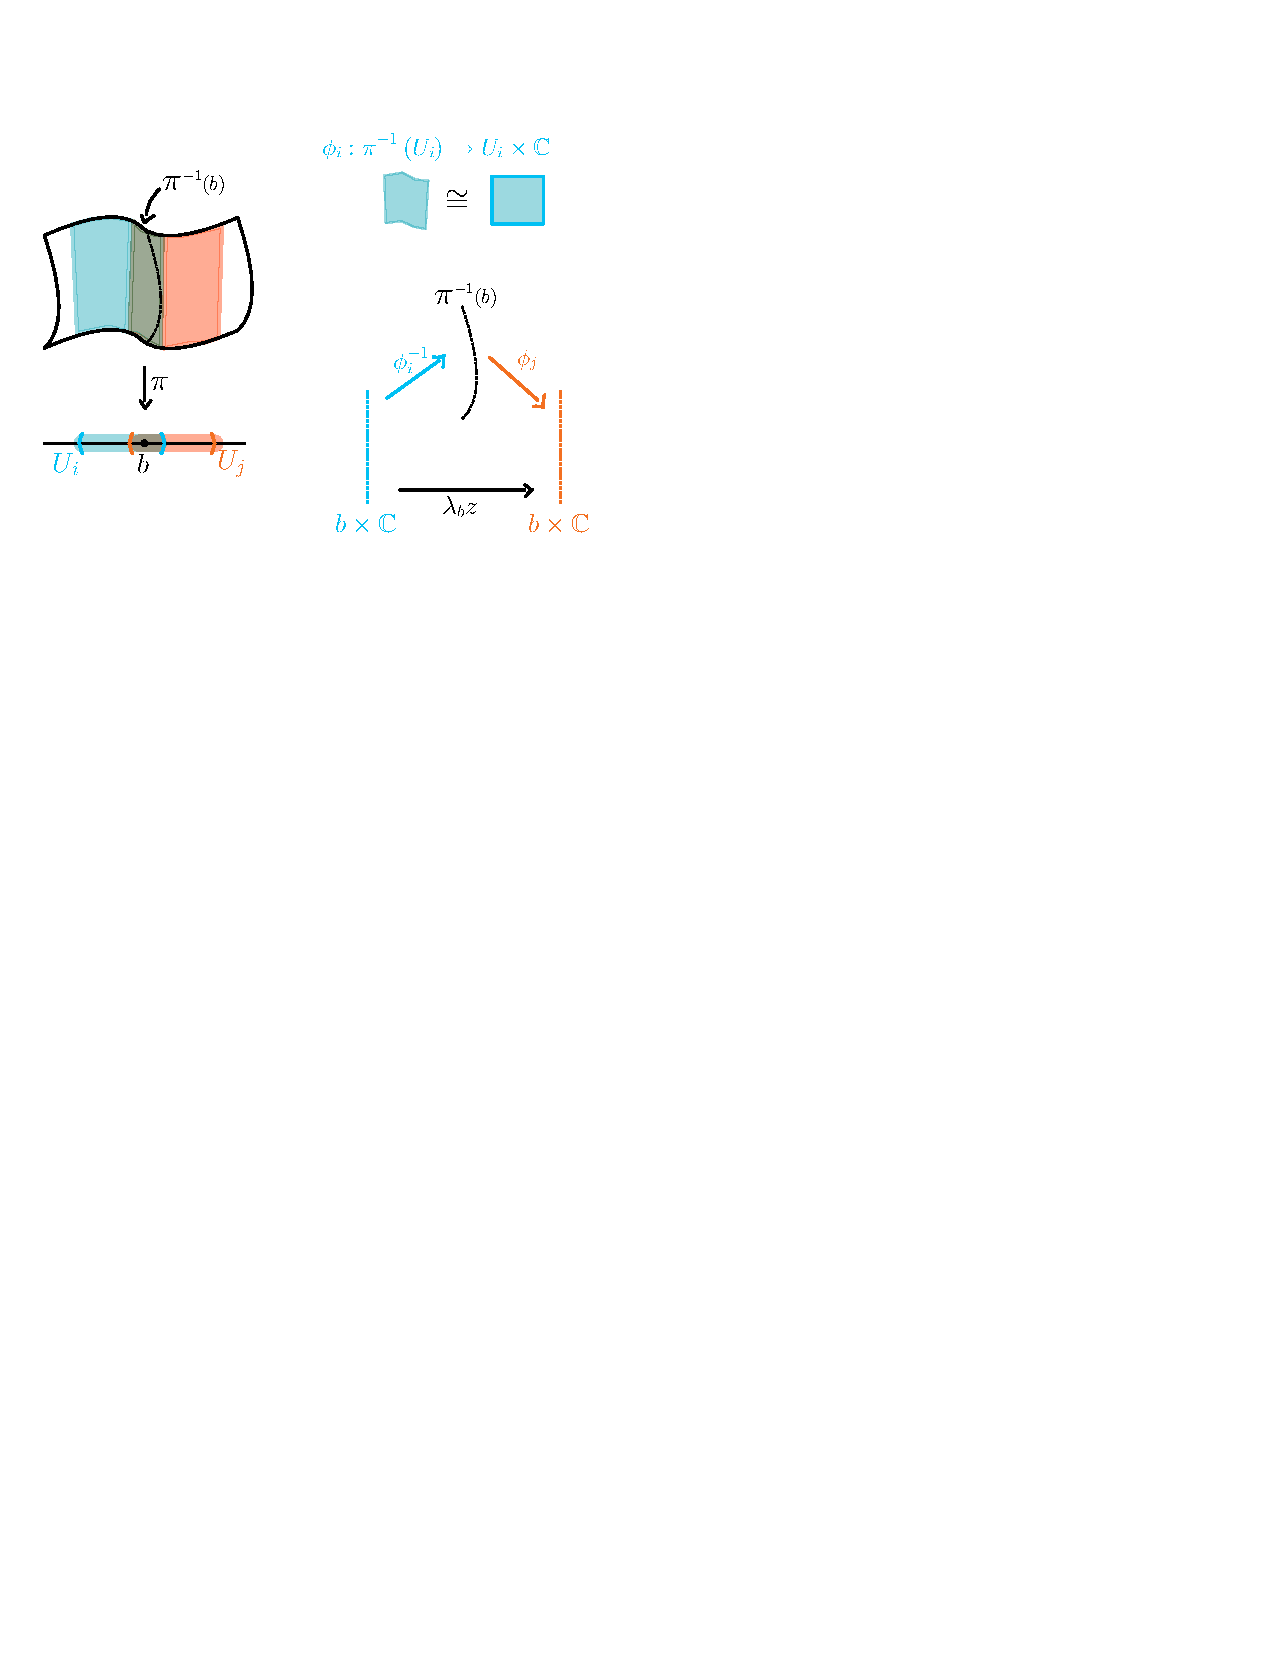
\includegraphics[width=0.8\textwidth, trim= 0.725cm 19.25cm 11.625cm 2.25cm,clip]{figs/figLineBundleDefn.pdf}
    \caption{Line Bundle with the two properties}
    \label{fig:2.1-LineBdlExample}
\end{figure} 

\begin{Def}
    A \term{section} of a line bundle $L$ over $B$ is a map $s\:B\to L$ with $\pi s=\id_B$. 
\end{Def}

Sections can be defined locally on open sets $U\subseteq B$ or globally when they are defined everywhere on $B$. Intuitively, a section singles out points in fibers. For every $b\in B$, $s(b)$ is a point on the fiber $\pi^{-1}(b)$.
\subsection*{The Fun Part is not the sets, it's the\dots}

\textbf{Base morphisms} of a families are maps between total spaces which carry fibers onto fibers and distiguished points to distinguished points. For the case of line bundles we have just a tiny bit more.
    
\begin{Def}
    A \term{morphism of line bundles} is a map $f\: L_1\to L_2$ which makes the following diagram commute:
    \begin{center}
        \begin{tikzcd}
            L_1 \arrow[rdd, "\pi_1"'] \arrow[rr, "f"] && L_2 \arrow[ldd, "\pi_2"] \\&&\\& B&
            \end{tikzcd}
    \end{center}
    It must hold that on fibers, the map $f$ restricts to a \textbf{linear map}.
\end{Def}

Unwrapping the definition a bit, we have that the diagram commutes when $\pi_1=f\pi_2$. So the question is, where does a point in a fiber, $x\in\pi^{-1}_1(b)$, map to? We would like it to be in the corresponding fiber of $L_2$.\par 
For $f(x)\in\pi_2^{-1}(x)$, it must occur that $\pi_2(f(x))=b$. But we have 
$$\pi_1(x)=\pi_2(f(x))\word{and}\pi_1(x)=b,$$
so it holds that 
$$f\left(\pi^{-1}_1(b)\right)\subseteq \pi_2^{-1}(b).$$
Similarly for sections for sections, the diagram commutes when $s_2=fs_1$. But this means that for $b\in B$, 
$$s_2(b)=f(s_1(b)),$$
so distinguished points of fibers get sent to the corresponding distinguished points.

\section{Line Bundles over $\bP^1$}

We begin by introducing a family of complex manifolds.

\begin{Def}
    The manifold $\cO_{\bP^1}(d)$ is defined by two charts and a transition function:
    $$(\bC^2,(x,u))\xrightarrow[v=u/x^d]{y=1/x}(\bC^2,(y,v)).$$
    This transition function is  $(y,v)=\left(\frac{1}{x},\frac{u}{x^d}\right)$ with inverse $\left(\frac{1}{y},\frac{y}{v^d}\right)$.
\end{Def}
We could also regard this set as $\bC^2$ under the equivalence relation described via the transition function.

\subsubsection{No other line bundles}
$\cO_{\bP^1}(d)$ comes with a natural projection onto $\bP^1$ 
$$(x,u)\mapsto x$$
This allows us to see $\cO_{\bP^1}(d)$ as a line bundle, because every fiber $\pi^{-1}(x)$ is isomorphic to $\bC$. When $x$ is non-zero we get a copy of $\bC$ on both charts, but when $x=0$ or $\infty$, the line is only on one of the charts.\par 
Spoiling ourselves of the fun\footnote{Because it'd be so much fun to prove this are all the line bundles.}, we claim that all line bundles over $\bP^1$ are of the form $\cO_{\bP^1}(d)$ for an integer $d$. 

\chapter{Premier on the Chow Ring by \emph{Richard E. Borcherds}}

\section{The Chow ring}

This summary is based on Richard E. Borcherds' introduction to the Chow ring in Youtube.

For a non-singular variety \( V \), we define the \emph{Chow ring} \( A^\ast(V) \), whose elements \emph{correspond} to subvarieties of \( V \), and the product reflects the intersection of these subvarieties. The ring is graded by codimension:
\[
A^\ast(V) = \bigoplus_i A^i(V)
\]
where \( A^i(V) \) consists of classes of subvarieties with codimension \( i \). Ideally, the intersection of a codimension \( m \) subvariety \( X \) and a codimension \( n \) subvariety \( Y \) would yield a subvariety of codimension \( m+n \). However, this does not always hold. Imagine a hyperplane $H$ intersected with itself. So there's a complication in defining this product.

\subsection{Cycles and Intersection Numbers}

An initial attempt to resolve starts by defining \emph{cycles}, which are formal sums of subvarieties. Specifically, we define the group of codimension \( i \) cycles as:
\[
A^i(V) = \left\langle X \mid X \subseteq V, \ \text{closed subvariety}, \ \codim(X) = i \right\rangle
\]
For two cycles \( X \in A^i(V) \) and \( Y \in A^j(V) \), we aim to define their product as:
\[
X \cap Y = \sum_{Z} i(X, Y; Z) Z
\]
where the sum runs over the irreducible components \( Z\) of \( X \cap Y \), and \( i(X, Y; Z) \) is an \emph{intersection number}, representing the multiplicity of the intersection at \( Z \). However, defining this intersection number precisely poses significant challenges.

\subsection{Rational Equivalence and the Chow Group}

To address the ambiguities in defining intersections, particularly when subvarieties do not intersect transversely, we use the notion of \emph{rational equivalence}. Cycles are considered equivalent if their difference is the divisor of a rational function on a subvariety of dimension \( j+1 \). This leads to the following definition:

\begin{Def}
The \( i \)-th \emph{Chow group} \( A^i(V) \) of a non-singular variety \( V \) consists of equivalence classes of codimension \( i \) cycles, where two cycles are equivalent if their difference is a principal divisor, i.e., the zero set of a rational function.
\end{Def}

The \emph{Chow ring} is the direct sum over all Chow groups:
\[
A^\ast(V) = \bigoplus_i A^i(V)
\]
The intersection product on the Chow ring is well-defined:
\[
[X] \cap [Y] = \sum_{[Z]} i(X, Y; Z) [Z]
\]
where \( [X] \), \( [Y] \), and \( [Z] \) denote rational equivalence classes of cycles.

\subsection{Example and Further Considerations}

\begin{Lem}[Chow's moving lemma (1956)]
Given two algebraic cycles $X,Y$ in $V$ a non-singular variety, there is another cycle $Y'$ rationally equivalent to $Y$ on $V$ such that $X$ and $Y'$ intersect \emph{properly}. \red{Look for better reference than wikipedia}.
\end{Lem}

Let's illustrate this by considering the next example.

\begin{Ex}
    Consider the surface $S=\Bl_{\text{pt}}\bP^2$. We have a copy of $\bP^1$ as the exceptional divisor $E$. If we ask what is $E\cap E$, then we have to move $E$ slightly.\par
    This is impossible as $E$ can't be deformed. This is not a counterexample to Chow's lemma but to see this we have be a bit subtle. Consider a line $A$ which we deform to pass about the exceptional divisor, call it $B$. This means that 
    $$A\sim B\cup E\To E\sim A-B.$$
    $A-B$ has a well-defined intersection with $E$ because $A$ doesn't meet $B$ and $B$ has a transversal intersection with $E$. Thus $(A-B)\cap E$ is well defined as we've deformed $E$ into a cycle with negative coefficients.\par
    Observe that if we deform $E$ to something which has transversal intersection with itself, we will acquire negative coefficients because 
    $$E\cap E=(-1)[\text{pt}].$$
    So we will acquire negative coefficients when turning $E$ into a well-behaved cycle.
\end{Ex}

In essence, Chow's lemma doesn't say we can deform subvarieties, it says we can deform cycles and even if we start with one with positive coefficients, we may end up with one with negative coefficients.\par 

Now if $V$ is a singular variety, we may end up with extra complications.

\begin{Ex}
    Suppose we take $V$ to be a cone and two subvarieties $X,Y$ being a hyperbola and a line through the singularity.
\red{Add figure}
    If we intersect $X\cap Y$ we get just one point without troubles, but let us slide $X$ so that $X$ becomes a \emph{double line} through the singularity. So it might the case that $X\sim 2Z$ where $Z$ is the corresponding line. It must happen as well that 
    $$2Z\cap Y=[\text{pt}]\To Z\cap Y =\half[\text{pt}].$$
    We can still get intersections on varieties with singularities but with rational coefficients.
\end{Ex}

This means that it certainly does make sense to consider the Chow ring of $\ov{M}_{g,n}$.

\begin{Qn}
¿Is this why there appears a $\frac{1}{24}$ in some places when doing calculations with $\la$-classes?
\end{Qn}

\begin{ptcb}[RQ 241212]
    It's actually not the $\la$ class, ¡but the $\psi$ class! The result I was remembering at that moment was 
    $$\int_{\ov M_{1,1}}\psi_1=\frac{1}{24}$$
\end{ptcb}

Finally, lets consider examples of Chow groups and Chow rings. In general finding the Chow ring is very hard, but we have
\begin{itemize}
    \item The $0^{\text{th}}$ Chow group, $A^0(V)\isom\bZ$, is generated by $[V]$. This is the class of the whole variety or \emph{the fundamental class}. This is the multiplicative identity in the Chow ring as $X\cap V=X$. 
    \item $A^1(V)$ contains hypersurfaces modulo linear equivalence. This are basically divisors up to linear equivalence which amounts to the Picard group of $V$, $\Pic(V)$. Already for an elliptic curve, $\Pic(V)$ is uncountable.
\end{itemize}

\begin{Ex}
    If $V=\bP^2$, then $A^{i}(V)\isom\bZ$ for $0\leq i\leq 2$. This is because we can decompose $\bP^2$ as 
    $$\bP^2=\text{pt.}\cup\text{line}\cup\text{plane}$$
    In general $A^\ast(\bP^n)\isom\bZ[H]/\genr{H}^{n+1}$ where $H$ represents the class of a hyperplane in $A^1(\bP^n)$.\par
    ¡This is the same case for the Grassmannian! Its Chow ring is also easy to describe as we may decompose the Grassmannian into affine spaces.
\end{Ex}

\begin{Qn}
    ¿What is the Chow ring of the Grassmannian?
\end{Qn}

\begin{Rmk}
    Some of this intersection numbers can also be calculated with Schubert calculus, and they happen to coincide with Littlewood-Richardson coefficients.    
\end{Rmk}

\begin{Ej}
    Consider the rational normal curve in $\bP^2$, $C=V(XY-Z^2)$. As a closed subvariety of $\bP^2$, $[C]\in A^1(\bP^2)$, which means $[C]=d[H]$ where $[H]$ is the class of a hyperplane. In $\bP^2$, $H$ is the class of a line.
    \begin{enumerate}
        \item ¿Can we form a conjecture about what the multiple of the hyperplane class will $[C]$ be intuitively?
        \item Show that $d=2$ by explicitly describing a rational map between $C$ and $2$ lines.
    \end{enumerate}
\end{Ej}

\begin{ptcb}
There was a way to go about the second item via the affine case, say the curve is $xy-1=0$ and we can take the two axes $x,y$ and then form the family of curves $xy=t$ with $t$ varying from $0$ to $1$. Then this, in some fashion, formed the desired rational map. \red{ASK RENZO}
\end{ptcb}

\begin{Ej}
    Generalize the previous exercise to the case of a degree $d$ curve in $\bP^2$. Also, ¿what happens if we consider the sum of different degree cycles? Say something like $3U+2V$, ¿what will be the multiple of the hyperplane class there?
\end{Ej}

\section{Chern classes}

\subsection{A quick cheat sheet}

Let us begin with the Chern class cheat sheet${}^{\text{TM}}$. This based off of my meeting with Renzo on 20240917. First assume $E\xrightarrow{\pi}B$ is a rank $r$ vector bundle. We have the following:

\begin{itemize}
    \item $c_i(E)\neq 0$ whenever $0\leq i\leq r$.
    \item $c_i(E)$ has degree $i$ in the Chow ring. This means $c_i(E)\in A^i(B)$.%A^i(E)$. (¿or $A^i(B)$?) It was the base all along. 
    \item $c_0(E)=1$, or in words, it's the fundamental class. It's usually the case that we rescale in order for this to be exactly $1$.
    \item If we define 
    $$c_{\text{tot}}=c_0+c_1+\dots+c_r$$
    and we have a short exact sequence of vector bundles 
    $$0\to F\to E\to Q\to 0,$$
    then $c_{\text{tot}}(E)=c_{\text{tot}}(F)\.c_{\text{tot}}(Q)$. In particular we have 
    $$c_1(E)=c_1(F)+c_1(Q).$$
    \item If $E$ is a line bundle $L$, i.e. rank 1, then 
    $$c_1(L)=[\div(s)],$$
    this is the class of the divisor of a meromorphic section.
    \item $c_1$ commutes with pullbacks.
\end{itemize}

For more, check out \href{https://math.stackexchange.com/questions/989147/quick-question-chern-classes-of-sym-wedge-hom-and-tensor}{this math.se post}\footnote{\href{math.stackexchange.com/q/989147/}{\ttt{math.stackexchange.com/q/989147/}}} or \href{https://rigtriv.wordpress.com/2009/11/03/chern-classes-part-1/}{here}\footnote{\href{https://rigtriv.wordpress.com/2009/11/03/chern-classes-part-1/}{\ttt{https://rigtriv.wordpress.com/2009/11/03/chern-classes-part-1/}}}.

\subsection{A Historical Note}

Continuing with Richard Borcherds' lecture, we focus on how to obtain Chern classes from a vector bundle $E\xrightarrow{\pi}V$ over a non-singular variety $V$. These are certain elements of $A^i(V)$

    On the side of historical notes, in differential geometry, Chern classes take values in the cohomology ring of $V$ when seen as a complex manifold. The Chow ring is related to the cohomology ring via a homeomorphism 
    $$A^i(V)\to H_{2n-2i}(V)\to H^{2i}(V)$$
    where the first map is taking a cycle to a cycle, and then applying Poincaré duality.
    
    \begin{Rmk}
        Personally, I believe it would be more accurate to say that the Chow ring is more closely related to homology groups than to cohomology. This is because cohomology deals with functions mapping cycles to $\bR$ while homology is primarily concerned with formal groups of cycles. 
    \end{Rmk}

    This map is not injective in general as $A^i(V)$ is hopelessly huge in general. For an elliptic curve $E$, it happens that 
    $$A^{1}(E)\word{is uncountable, but}H^{2}(E)=\bZ.$$
    It is also not onto as nothing in the Chow ring maps to $H^{2i+1}(V)$ for any $i$. We may refine our question to 
    $$\text{¿is}\quad A^i(V)\to H^{2i}(V)\quad\text{onto?}$$ 
    And the answer remains negative. The image of this map is subtle, and Hodge established that
    $$H^{2i}(V,\bR)\isom\bigoplus H^{p,q}(X)\word{and}\Im(A^i)\subseteq H^{i,i}(V).$$
    So the previous question can be further refined to, 
    $$\text{¿is}\quad \Im(A^i)=H^{i,i}(V)\cap H^\ast(X,\bZ)?$$
    Once again not positive. Atiyah and Hirzebruch found a torsion element in the cohomology that is not in the image of $A^i(V)$. This leads us to the Hodge conjecture which remains unsolved. 

\subsection{Characteristic Classes}

\begin{Ex}
    For a line bundle $L\xrightarrow[]{\pi}B$, take a section $f$. So at each point $b\in B$, $f$ picks out a point in the fiber $\pi^{-1}(b)$. Usually the set of zeroes of $f$ is a codimension $1$ cycle of $B$.
    \begin{center}
        \red{add drawing}
    \end{center}
    This cycle lives in $H_{n-1}(B)$ where $\dim B=n$. Via Poincaré duality, this gives us an element in $H^1(B)$. This is the first Stiefel-Whitney class of $L$.\par
    If we take $B=S^1$, we have two obvious line bundles, $S^1\x\bR$ and the Möbius bundle. 
    \begin{center}
        \red{add drawing}
    \end{center}
    In the case of the trivial bundle, the zeroes of a non-zero section will always be even, while in the case of the Möbius bundle, it'll always be odd. This means that at the level of $H^{1}(S^1,\bZ/2\bZ)$ we always get the $0$ and $1$ elements respectively. So we can distinguish this line bundles by counting the zeroes of a generic section.
\end{Ex}

The idea of characteristic classes is a generalization of this ideas. If we have a vector bundle, we can look at a section's zeroes and they will give us homology (or cohomology) classes.

\subsection{A First Step into Complex Land}

Chern classes on a complex vector bundle will take values in $A^*(V)$ (or $H^\ast(V)$ if we are doing differential geometry).\par
Consider a complex line bundle $L\xrightarrow[]{\pi}V$ over a non-singular variety or complex manifold $V$. We take the set of zeroes of a section $f$. This has complex codimension $1$ in $V$ and means that we have an element of $A^1(V)$, or in the real case, codimension $2$ with it being an element of $H_{2n-2}(V)\isom H^2(V)$.\par 
So the first Chern class is given by the cycle of zeroes of a section. We denote it $c_1(V)$.

\begin{Ex}
    ¿What is $c_1$ of $\cO(-1)$, the tautological bundle of $\bP^1$? We know that $\cO(-1)$ possesses no non-zero sections. But this is not a problem, as we may use the fact that 
    $$c_1(L\ox L')=c_1(L)+c_1(L')$$
    so we can tensor $\cO(-1)\ox\cO(d)$ for a sufficiently large $d$. This will be a line bundle with enough sections (\emph{hopefully}) so that $c_1$ makes sense here. In this case we define 
    $$c_1(\cO(-1))=c_1(\cO(-1)\ox\cO(d))-c_1(\cO(d)).$$
\end{Ex}

\subsubsection{More analytically, but not algebraically}
Another way to get $c_1$, we have the sequence of sheaves 
$$0\to\un{\bZ}\to\cO\xrightarrow{\exp}\cO^\ast\to 1$$
which only works in complex analytic geometry. So in terms of the long exact sequence of cohomology we have 
$$\dots\to H^1(V,\cO^\ast)\xrightarrow{c_1}H^2(X,\bZ)\to\dots$$
where the first term \emph{classifies} line bundles and the connecting morphism is more or less the first Chern class. 

\subsection{Higher Chern classes}

Returning to our vector bundle $E\xrightarrow{\pi}V$ of rank $r>1$, we follow Grothendieck's approach. We can associate $E$ with the projective bundle $P(E)$ where the typical fiber is isomorphic to $\bP^{r-1}$. Now $P(E)$ has itself a line bundle $\cO(1)$ leading us to a Chern class $c_1(\cO(1))\in A^1(P(E))$ which is not in $A^1(V)$. Thus, we must relate $A^\ast(P(E))$ with $A^\ast(V)$.\par
Call $H=c_1(\cO(1))$, the \term{hyperplane class}, to simplify notation. The Chow ring $A^\ast(P(E))$ forms a free, rank $r$ $A^\ast(V)$-module with basis $\set{1,H,\dots,H^{r-1}}$. This modularity arises from a similar reasoning to the construction of the Chow ring of $\bP^n$, which corresponds to the case when $V$ is a point. Now the element $H^r$ can be expressed as a linear combination of the basic elements: 
$$H^r=c_1H^{r-1}-c_2H^{r-2}+\dots\pm c_r,\word{for some}c_i\in A^i(V).$$
¡These coefficients are the Chern classes in $A^\ast(V)$! The class $c_r$ can be described easily. It is represented by a cycle of the zeroes of a section of $E$. The zeroes of that section will generally have codimension $r$ and we will be able to represent it by $c_r$.\par

Anticlimatically, we will call it the Euler class of our vector bundle. The reason we name it is because it's the only other Chern class that we can naturally give a description of.

\begin{Def}
    For a vector bundle $E\xrightarrow{\pi}V$ of rank $r\geq 1$, the \term{Euler class} is 
    $$e(E)\defeq c_r(E)=\bonj{\div(s)},$$
    the class of a divisor of a section.
\end{Def}

\begin{Rmk}
    ¡This is familiar! It generalizes the case of line bundles when $r=1$ as $e=c_1$. Recall that $c_1(\cO(-1))$ is $-\bonj{\text{pt}.}$ but we could pick a section and the cycle will change. If we pick a section with $20$ poles and $19$ zeroes then the divisor of that section is also $c_1$.
\end{Rmk}

\section{Intersections and the role of the Euler class}

This will summarize my meeting with Renzo from two weeks ago, on 20241001.

\subsection{Transverse Intersections}

\begin{Def}
    Let $X, Y \subseteq Z$. We say that $X$ and $Y$ intersect transversely at a point $p \in X \cap Y$ if 
    \[
    T_p Z = T_p X + T_p Y.
    \]
\end{Def}

\begin{Ex}
    Consider $X$ as a line and $Y$ as a plane in $\mathbb{R}^3$ such that $X$ is not contained in $Y$ (but not parallel to it). In this case, $X$ and $Y$ intersect transversely since their tangent spaces, $\mathbb{R}$ and $\mathbb{R}^2$ respectively, sum to $\mathbb{R}^3$ at the intersection point.
\end{Ex}

Note that the sum of the tangent spaces need not be a direct sum, as illustrated in the following example:

\begin{Ex}
    Let $\pi_1$ and $\pi_2$ be two planes in $\mathbb{R}^3$. Their intersection is a line. Each plane contributes two independent directions to their tangent spaces. Together, these directions span all of $\mathbb{R}^3$, meaning that the intersection is transverse.
\end{Ex}

We also have the following result:

\begin{Prop}
    If $X$ and $Y$ intersect transversely, then
    \[
    \bonj{X \cap Y} = \bonj{X} \. \bonj{Y} \quad \text{and} \quad \codim(X \cap Y) = \codim(X) + \codim(Y).
    \]
\end{Prop}

\subsection{Non-transverse intersection}

Let's begin with an example which lies in our minds to introduce non-transverse intersections. 

\begin{Ex}
    Consider the plane and line defined by 
    $$
    \left\lbrace
    \begin{aligned}
    &\pi=\set{3x+4y+6z=12}=\set{s(4,0,-2)+t(0,3,-2)+(0,0,2)}.\\
    &\l=\set{t(4,0,-2)+(0,0,2)}.
    \end{aligned}
    \right.
    $$
    We have that $\l\subseteq\pi$. So to follow the previous idea in transverse intersections we have two choices:
    \begin{itemize}
        \item Think like a topologist and wiggle $\l$ until becomes transverse with $X$, but watch out, we wouldn't like to wiggle it completely inside of $X$.
        \item Think like an algebraic geometer and replace $\l$ with an equivalent transverse cycle. This idea uses Chow's moving lemma!
    \end{itemize}
    The smart topologist wishes to wiggle $\l$ outside of $\pi$, this is done through the normal bundle of $\pi$ inside of $\bR^3$. Observe quickly that this bundle is the collection of normal spaces of points of the plane. For $P\in\pi$ we have
    $$N_P(\pi)=\set{x\in T_P(\bR^3)\:\ \braket{x}{y}=0,\quad y\in T_P(\pi)}$$
    where $T_P(\bR^3)$ is the whole of $\bR^3$ and $T_P(\pi)$ is $\pi$ but parametrized as 
    $$T_P(\pi)=\set{u(4,0,-2)+v(0,3,-2)+P}.$$
    In any case the normal space is spanned by the vector $(3,4,6)$ so that at point $P$, the normal space is $\set{t(3,4,6)+P}$. Restricting it to $\l$ we obtain the wiggle room, the normal bundle 
    $$N_{\pi\subseteq\bR^3}\mid_{\l}=\set{N_P(\pi)\:\ P\in\l}.$$
    Wiggling $\l$ across the normal bundle gives us a \emph{section} of the normal bundle. First of all, \red{finish}
\end{Ex}

\chapter{Graphs and Chapter 1 of \emph{The Green Book}}

\section{Dual graphs}

Let us recall an important definition:

\begin{Def}
    A \term{stratum} in $\ov{M}_{g,n}$ is the closure of the set of all curves with the same topological type. Strata are classified by dual trees. 
\end{Def}

\begin{Ex}
    In $\ov M_{0,6}$, the fundamental class $1\in A^0(M_{0,6})$ is the class of all curves homeomorphic to a 6-pointed $\bP^1$. It can be represented by the dual graph:\par
    \begin{figure}[h!]
        \centering
        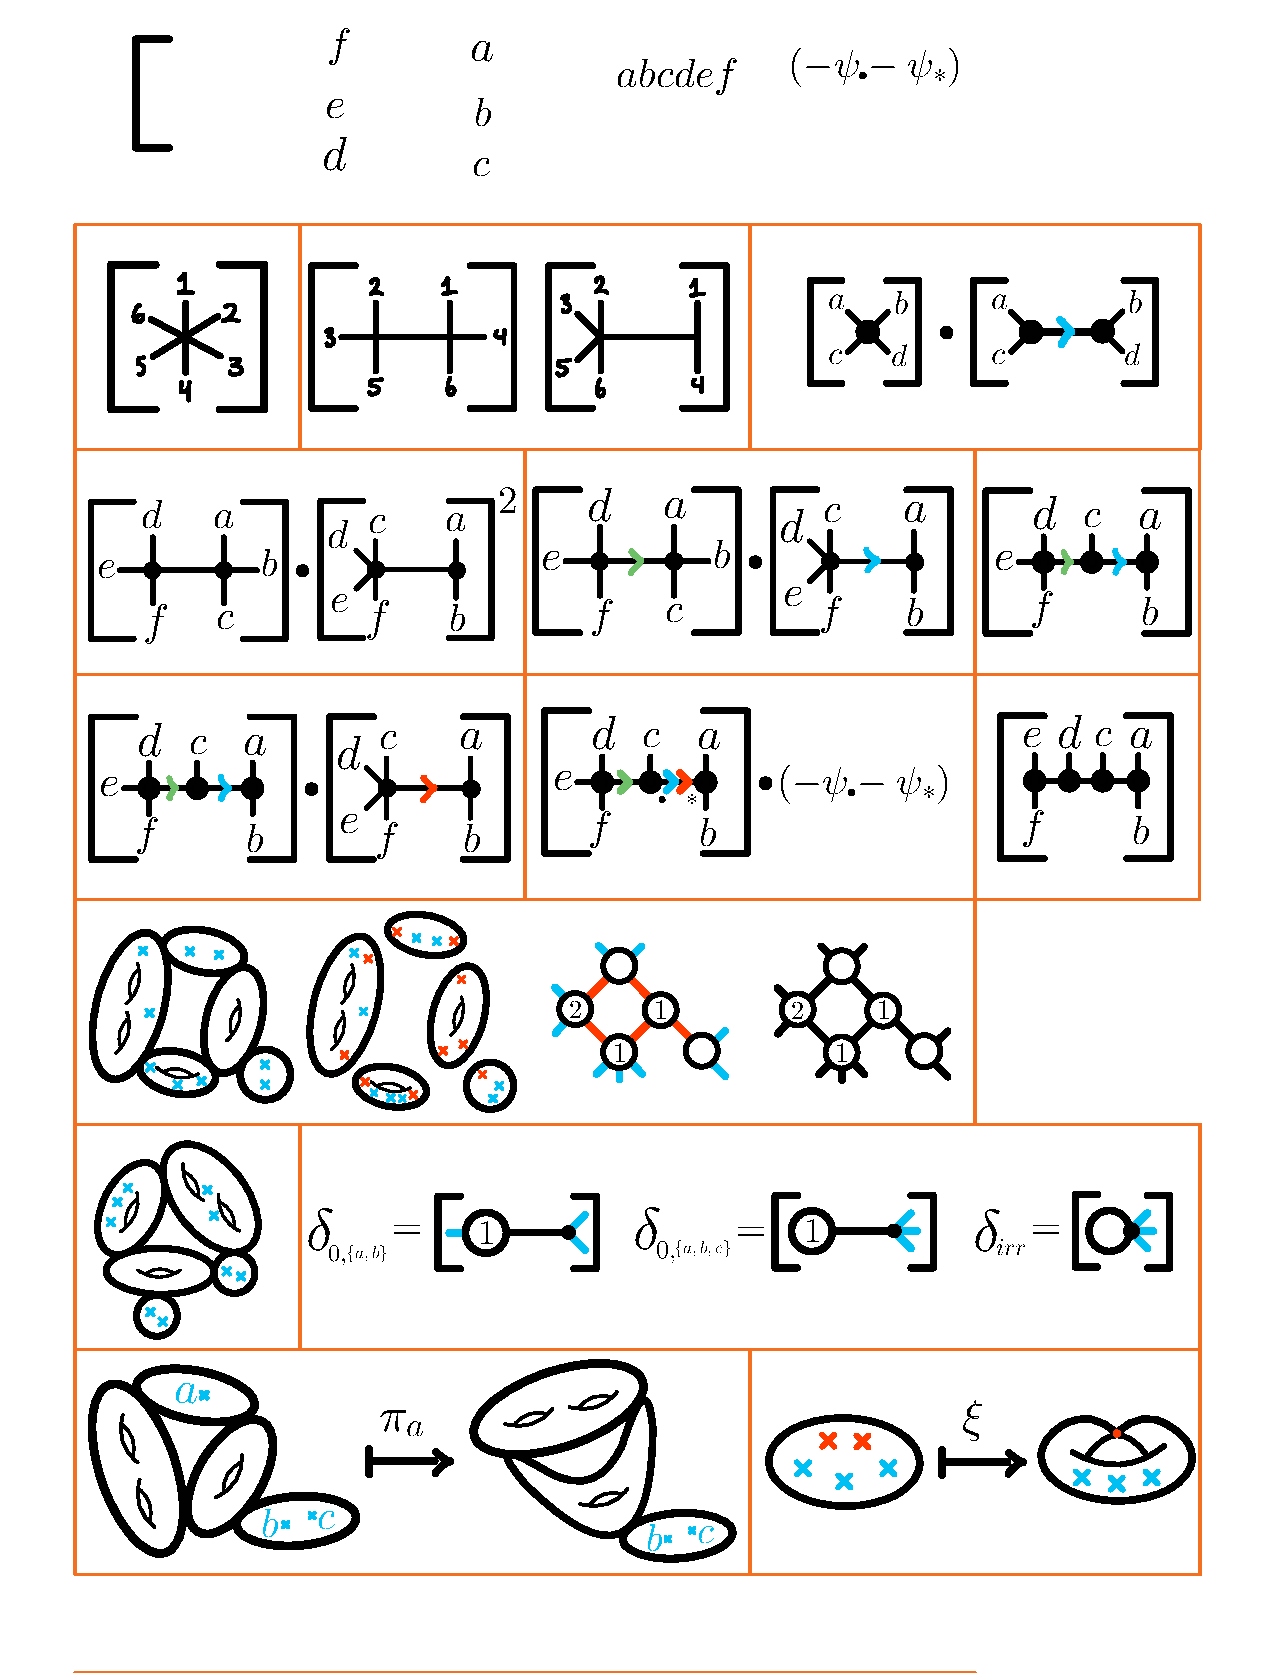
\includegraphics[width=0.2\textwidth, trim= 1.32cm 20.75cm 16.53cm 3.9cm,clip]{figs/FigsDNnotability1.pdf}
        \caption{Fundamental class representative of $\ov{M}_{0,6}$}
        \label{fig:3.1-fundamental class}
    \end{figure} 
    The top stratum in $\ov M_{0,6}$ contains only one topological type of curve as all other $6$-pointed $\bP^1$'s will be homeomorphic to this one.
\end{Ex}

\begin{Ex}
    Going into the boundary of $\ov M_{0,6}$ we can find two different types of strata, for example
    \begin{figure}[h!]
        \centering
        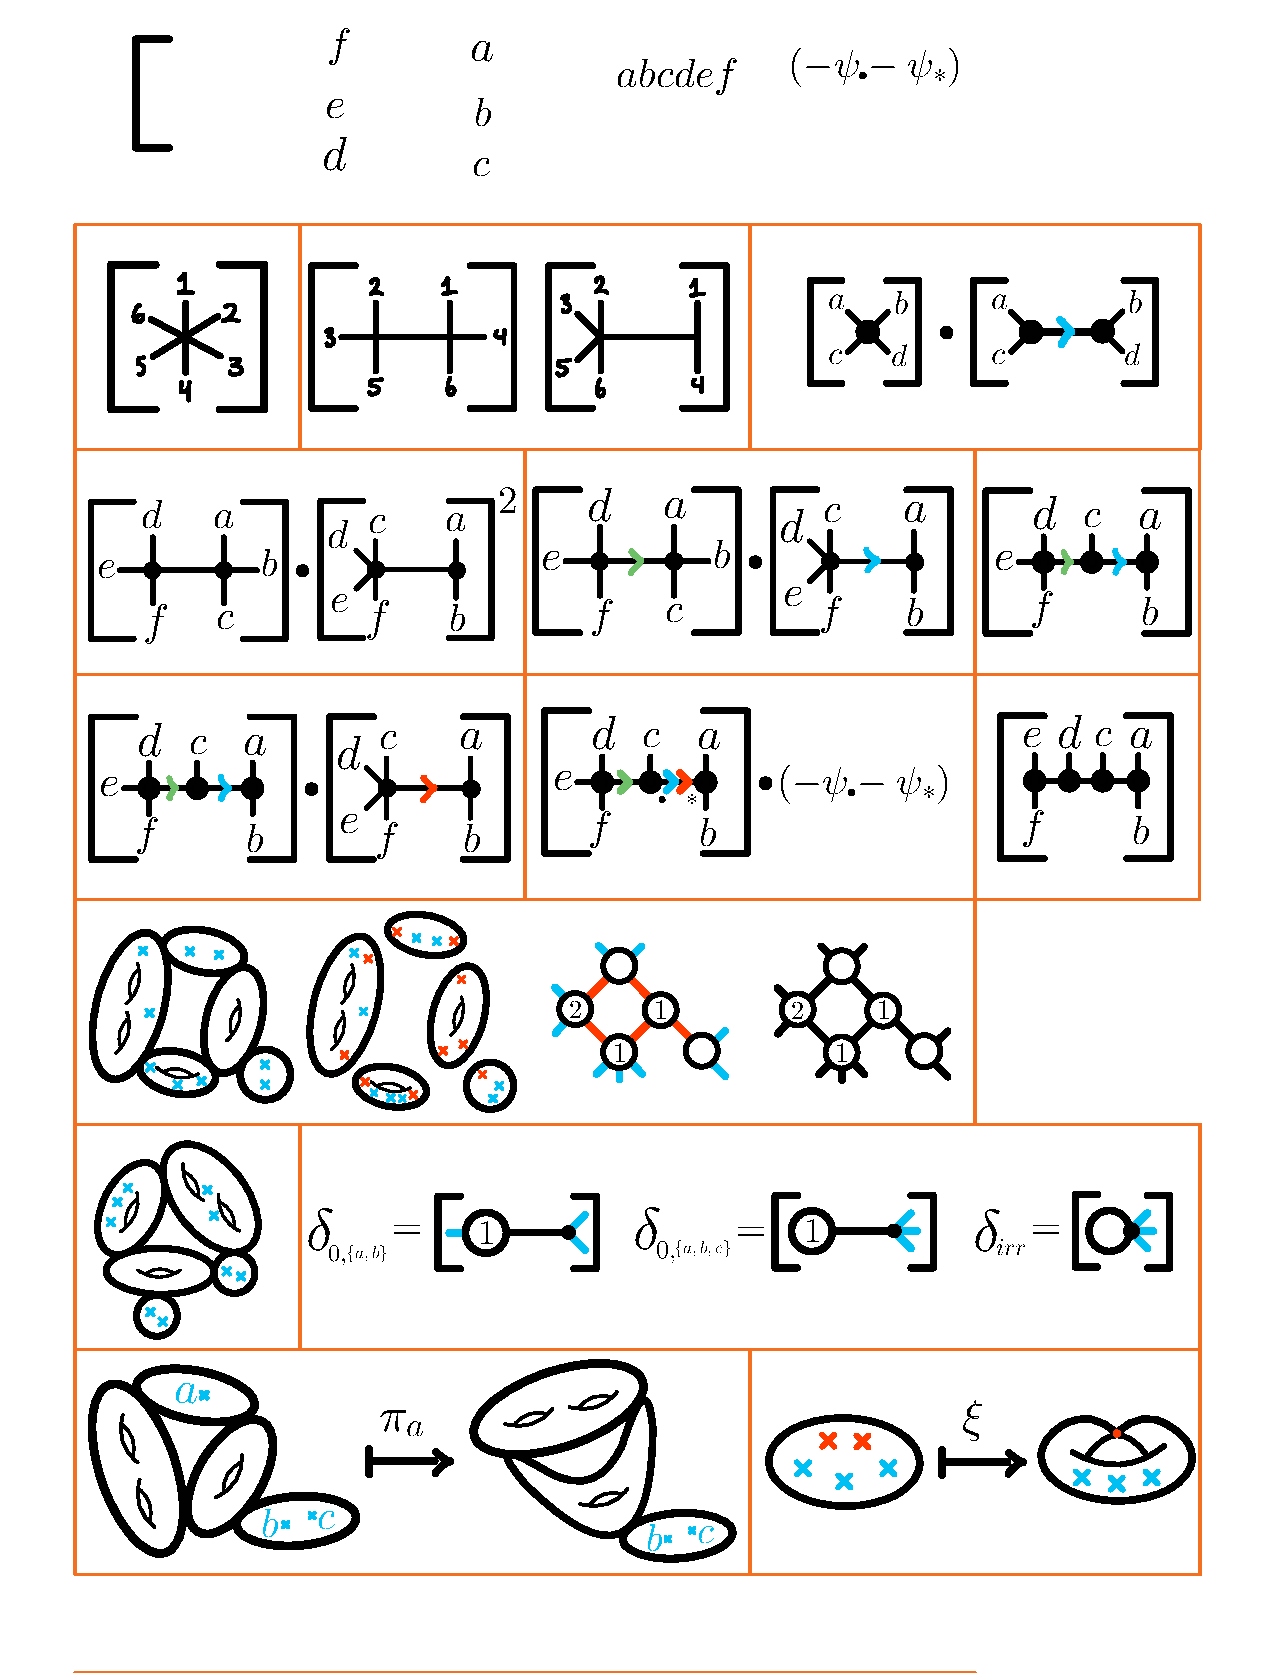
\includegraphics[width=0.4\textwidth, trim= 5.12cm 20.75cm 8.93cm 3.9cm,clip]{figs/FigsDNnotability1.pdf}
        \caption{Examples of boundary strata of $\ov{M}_{0,6}$}
        \label{fig:3.2-boundary-strata-M06c1}
    \end{figure} 
    From the stratum on the left, we can find $9$ other strata with the same graph design but different labelings. This is because there are 
    $$\half\binom{6}{3,3}=\frac{6!}{2\.3!\.3!}=10$$
    ways to label the tree. The factor of $\half$ accounts for the symmetry in the tree.\par
    For the one on the right we can find $\binom{6}{4,2}=15$ labelings.
\end{Ex}

\begin{Def}
    Boundary cycles of codimension one in $\ov M_{g,n}$ are called \term{boundary divisors}. These can be denoted $D(I\mid J)$ where $I,J$ is a partition of $\bonj{n}$ and $|I|,|J|\geq 2$.
\end{Def}

\begin{Ex}
    For simplicity, the previous boundary divisors can be named $D(235\mid 146)$ and $D(2356\mid 14)$.
\end{Ex}

\begin{Prop}
    There are 
    $$\half\sum_{k=2}^{n-2}\binom{n}{k}=2^{n-1}-n-1$$
    irreducible boundary divisors in $\ov M_{0,n}$.
\end{Prop}

\begin{ptcbp}
    A partition into two sets of $\bonj{n}$ of size $k$ and $n-k$ can be done in $\binom{n}{k,n-k}$ ways. Observe that this coefficient is precisely $\binom{n}{k}$. We need to divide by 2 because $\binom{n}{k}=\binom{n}{n-k}$. And as we need $2\leq k\leq n-2$ for the curve to be stable, we must sum over all of those possibilities. 
\end{ptcbp}

\subsection{Products of cycles as graphs}

In order to find the intersection product of two cycles we do the following:

\begin{enumerate}
    \item Find the dual graphs corresponding to the cycles.
    \item Paint the edges of both graphs with \emph{oriented} colorings $c_1,c_2$. 
    \item Compute the codimension of the product, recall codimension is the number of edges.
    \item The resulting graphs, should have no more edges than the expected codimension.
    \item Consider all graphs which contain the factors' dual graphs as minors\footnote{The current lingo in geometry is specialize.} at the same time.
    \item Color the edges of the resulting graphs such that when collapsing edges, the original coloring of a factor is obtained. No edge of a resulting graph may be left \textbf{uncolored}.
    \item If an edge is bicolored multiply the corresponding $\psi$-classes. 
    \item Count number of automorphisms of the graph and divide the class by that number. 
    \item Count the number of possible colorings which respect the conditions and multiply the class by that number.
\end{enumerate}

\begin{Rmk}
    When we think we have a graph but it doesn't match the conditions in the end, we say that it is a \term{non-generic intersection}. That might occur because it leaves in a lower codimensional strata.
\end{Rmk}

In summary, the formula for the intersection product is as follows:

\begin{Prop}\label{prop-intersection-prod-formula-for-dual-graphs}
    For two curves $C_1,C_2$ whose dual graphs are $\Ga_1,\Ga_2$ we have that the class of their intersection product has dual graph:
    $$\Ga_1\.\Ga_2=\sum_{\Ga\supseteq\Ga_1,\Ga_2}\frac{(\#\text{ colorings})}{|\Aut(\Ga)|}\.\Ga\.\prod_{i}(-\psi_{\8 i}-\psi_{\star i}),$$
    where the sum runs through graphs $\Ga$ containing $\Ga_1,\Ga_2$ as minors, the number of colorings is the amount of colorings which respect the edge-contraction process, and the product of $\psi$-classes runs through the amount of bicolored edges.
\end{Prop}


\subsection{Computations of Intersection Products}
This becomes clearer when doing examples:

\begin{significant}
    What I hear, I forget;\par
    When I see, I remember;\par
    When I do, I learn.\par
    -Some Chinese fella
\end{significant}

\begin{Ex}
    Let's begin with a sanity check. Consider the product in $\ov M_{0,4}$ of the fundamental class with $D(ac\mid bd)$. The classes in graph form are the following:\red{Add drawing}.\par
    Let's proceed by following the algorithm:
    \begin{itemize}
        \item We have found the graphs and now we color. The fundamental class has no edges, we do not color. Whereas $D(ac\mid bd)$ has one edge which we choose to color as we showed.
        \item The codimension of this product should be 1. There's only one edge in total and the result shouldn't have more than one edge.
        \item Many graphs contain our factors as minors:\red{Add drawing}.\par
        But, as in the case of this one, they might not be stable. And even if they were, observe that a graph like this one has 3 edges, 2 of which we can't color. Recall, the cases when the graph is \emph{actually stable} but it can't be colored it's a non-generic intersection.\par
        The only graph which contains then, both of our factors is the dual graph of $D(ac\mid bd)$. It can only be colored in the way that respects the coloring of the factor.
        \item No edges are multicolored and in this case there's no automorphisms nor different colorings.
    \end{itemize}
    Therefore it happens that:
    $$1\.D(ac\mid bd)=D(ac\mid bd)$$
    as expected.
\end{Ex}

\begin{Ex}
    Consider now the product $D(ac\mid bd)^2$ in $\ov{M}_{0,4}$. As this boundary divisor has codimension $1$, its square should have codimension $2$.\par
    ¡But $\ov{M}_{0,4}$ has only one dimension! It must follow that the product is empty.\par
    To see this via the algorithm, we consider all graphs containing $D(ac\mid bd)$ as a minor. There's no graphs with two edges as that violates the stability condition (all vertices should have at least 3 special points), and so the only possible graph is a copy of $D(ac\mid bd)$ with its only edge bicolored.\red{Add drawing}.\par
    Label the marks $\ast$ and $\.$ on the edge of $D(ac\mid bd)$ so that we may see this class as the image of the gluing morphism 
    $$gl\: M_{0,\set{a,c,\ast}}\x M_{0,\set{b,d,\.}}\to M_{0,4}.$$
    Then the $\psi$-classes we muliply are $(-\psi_{\.}-\psi_{\ast})$ so that the result is $D(ac\mid bd)\.(-\psi_{\.}-\psi_{\ast})$.\red{Add drawings}\par
\end{Ex}

\begin{ptcb}
    \begin{Qn}
        How was the process of saying that this intersection was zero by distributing the psi class into the $M_{0,3}$'s or something?
    \end{Qn}    
\end{ptcb}

Let's go up some dimensions

\begin{Ex}
    Consider the intersection product in $\ov{M}_{0,6}$:
    $$D(abc\mid def) D(ab\mid cdef)^2 $$
    The corresponding dual graphs are \red{Add drawings}\par
    The expected codimension of the result is $3$ as every factor contributes $1$ codimension.\par

    We first multiply a copy of $D(ab\mid cdef)$ with $D(abc\mid def)$:\red{add drawing with edges colored}.\par

    Graphs which contain these two as minors are scarce. In fact, ¡there's only one: $D(ab\mid c\mid def)$!\red{add drawing}\par 

    We get only one copy of our resulting graph with the coloring already determined.
    This graph has no non-trivial automorphisms and so we only get $D(ab\mid c\mid def)$ which we now have to multiply by another copy of $D(ab\mid cdef)$.\red{add drawing with edges colored}.\par

    We expect the resulting graphs to have three edges as that would have codimension $3$. But take for example $D(ab\mid c\mid d\mid ef)$. \red{add drawing with edges colored}.\par
    
    Such graph has three edges but \textbf{they can't be colored}. When collapsing edges, the colors disappear so that we would have to leave the edge between $d$ and $ef$ uncolored to respect the coloring.\red{Add drawing}\par
    This cannot happen as is the case for any other possibilities, they will be non-generic intersections. So $D(ab\mid c\mid def)$ is the only possible factor. The edge between $ab$ component and the $c$ component will be bicolored in a way that we have to multiply $\psi$-classes. Labeling the vertices attached to the edge as $\.$ and $\star$ we get 
    $$D(ab\mid cdef)^2 D(abc\mid def)=D(ab\mid c\mid def)(-\psi_\.-\psi_\star).$$
    This class has the correct codimension as the graph has two edges and the $\psi$ class adds another codimension.
\end{Ex}

\begin{Qn}
    ¿Is there a way to concretely determine whether a strata belongs in another one only by looking at their dual graphs?
\end{Qn}

\begin{Ex}[$(4,0)$ instead of $(0,4)$]
    Consider the curves represented by the following dual graphs:\red{add drawing}\par
    We have already colored them and now, very carefully, look at graphs which contain these ones as minors. 
    \begin{enumerate}
        \item The first graph itself has the second factor as a minor. We can color it in the following way:\red{add drawing with edges colored}.
        \item The following is a path graph which might appear to have many symmetries, but when imposing the coloring, we are left with only one copy of its class: \red{add drawing}\par
        This is because the two possible colorings and the reflection symmetry across the vertical axis cancel each other out. So in total we get a coefficient of $\half\.2=1$ accompanying it.
        \item Finally we get a star graph with a reflection across the axis which has the higher genus vertex.\red{add drawing}\par
        In the same fashion as before, that symmetry cancels the two possible colorings leaving us with only one copy of its class.
    \end{enumerate}
    There are no more graphs satisfying the required conditions\footnote{And if you claim to find one, try checking if you actually left edges uncolored or if it has the correct codimension.}. As the first term had a bicolored edge, we multiply by the corresponding $\psi$ class and write down the answer as follows: \red{add drawing}.
\end{Ex}

\begin{Ex}[Unexpectedly zero...]\label{ex-unexpectedly-zero-square}
    The following graph represents a curve in $\ov{M}_{1,2}$:\red{add drawing}\par
    Let us take its second power and color each factor's edge \green{green} and \blu{blue} respectively:\red{add drawing w edges colored}\par
    Following the process we now look for graphs which have this graph as a minor.
    \begin{itemize}
        \item The same graph certainly contains itself. But we must multiply by a $\psi$ class to get the correct codimension\red{add drawing w edges colored}\par
        Counting possible colorings we get 4 (\red{ask}) colorings and 2 automorphisms for this graph.
        \item The other curve consists of a torus twice-pinched with a mark on each of the isomorphic $\bP^1$ components. The dual graph looks like this:\red{add drawing w edges colored}\par
        It has quite a bunch of colorings, 8 and only two automorphisms.
    \end{itemize}
    So in total, the square of this curve can be represented by the sum of classes:\red{add drawings}
\end{Ex}

¿Why did I say that the previous class in example \ref{ex-unexpectedly-zero-square} is unexpectedly zero? It all has to do with\dots

\red{¿Do I move the lambda class example from MattAndRenzo here? Do I add a "other cohomology classes" section and then the MattAndRenzo example?}

\section{Integration}

My reference for this definition is Fulton and Pandharipande\cite{FPNotes}.

\begin{Def}[\cite{FPNotes} pg. 2]
    For a complete \red{In which sense? Cauchy sequences? Is it a Cauchy space\footnote{\href{https://en.wikipedia.org/wiki/Cauchy_space}{insane (clicky clicky)}}} variety, $c\in A^\ast(X)$ and $\bt\in A_k(X)$ then 
    $$\int_\bt c=\deg(c_k,\bt)$$
    where $c_k$ is the component of $c$ in $A^k(X)$ and $(c_k,\bt)$ is the evaluation of $c_k$ on $\bt$ giving us a zero cycle. When $V$ is a closed, pure-dimensional \red{can a class $\bt$ not be closed or pure-dimensional?} subvariety of $X$, then we write 
    $$\int_V c\word{instead of}\int_{\bonj{V}}c.$$
\end{Def}

Let us at once clear the idea of the squares-to-zero example \ref{ex-unexpectedly-zero-square}:

\begin{Ex}
    Let $\al$ by the curve in question for example \ref{ex-unexpectedly-zero-square}. We are interested in computing 
    $$\int_{\ov{M}_{1,2}}\al^2.$$
    We have that 
    $$\al^2=2\al(-\psi_{\81}-\psi_{\star1})+4\bt.$$
    Recall that the dimension of $\ov{M}_{1,2}$ is 
\end{Ex}
\section{Incursion into Pseudo-Stable Land}

Theorem 3.1 in MattAndRenzo \cite{MattAndRenzo} deals with the Mumford formula. This is the product of the total Chern class of the Hodge bundle over $\ov{M}_{g,n}$ with the one of the dual. The formula itself is 
$$(1+\hat{\la}_1+\dots+\hat\la_g)(1-\hat{\la}_1+\dots+(-1)^g\hat\la_g)=\sum_{i=0}^g\frac{1}{i!}\cG_\ast^i\left(\prod_{j=1}^i(\psi_{\star j}-\psi_{\8 j})\right).$$

To prove the formula we will do examples first. The first case that we deal with is in $\ov M_{1,n}$ for a fixed $n\geq 1$.

\begin{Ex}
    The pseudo stable Mumford formula in this case states:
$$(1+\hat{\la}_1)(1-\hat{\la}_1)=\frac{1}{0!}\cG_\ast^0\left(\id\right)+\frac{1}{1!}\cG_\ast(\psi_{\star 1}-\psi_{\8 1}).$$
    Let us analyze the left side. By definition, the pseudo-stable lambda class is 
    $$\hat\la_j=\cT^\ast(\la_j)=\sum_{i=0}^j\frac{1}{i!}\cG_\ast^i(p_0^\ast(\la_{j-i}))$$
    so in the case of $\hat\la_1$ we have 
    $$\hat\la_1=\sum_{i=0}^1(\dots)=\cG_\ast^0(p_0^\ast(\la_{1-0}))+\cG_\ast^1(p_0^\ast(\la_{1-1}))$$
    where $\cG^0$ is the identity map and $\la_0$ is the fundamental class of $A^\ast(\ov M_{g,n})$. So using this we have 
    \begin{align*}
        \hat\la_1&=\cG_\ast^0(p_0^\ast(\la_{1}))+\cG_\ast^1(p_0^\ast(\la_{0}))\\
        &=\la_1+\cG_\ast^1(\id)
    \end{align*}
    and expanding the product we get 
    \begin{align*}
        (1+\hat{\la}_1)(1-\hat{\la}_1)&=(1+\la_1+\cG_\ast^1(\id))(1-\la_1-\cG_\ast^1(\id))\\
        &=(\La_1(1)+\cG_\ast^1(\id))(\La_1(-1)-\cG_\ast^1(\id))\\
        &=\La_1(1)\La_1(-1)-\La_1(1)\cG_\ast^1(\id)+\cG_\ast^1(\id)\La_1(-1)-\left(\cG_\ast^1(\id)\right)^2.
    \end{align*}
    Here, $\La_1$ represents the total Chern class. We may analyze term by term this expression:
    \begin{itemize}
        \item The product $\La_1(1)\La_1(-1)=1$ is the usual Mumford formula. 
        \item For the case $\La_1(1)\cG_\ast^1(\id)$ what we have is $(1+\la_1)\cG_\ast^1(\id)$.
    \end{itemize}
    We now arrive to the question of what is $\cG_\ast^1(\id)$ so let's take a step back and remember how $\cG^1$ works as a map:
    $$\cG^1\: \ov M_{(1-1),n+1}\x\ov M_{1,1}\to \ov M_{1,n},$$
    and recall that the $\id$ in the argument is $p_0^\ast(\la_0)$ where the $\la_0$ comes from the Chow ring of $\ov M_{0,n+1}$. In particular, it is the fundamental class of the space. Pulling it back just makes it part of an ordered pair and then pushing it forwards attaches it to a copy of an elliptic curve. Graphically:
    \begin{figure}[h]
        \centering
        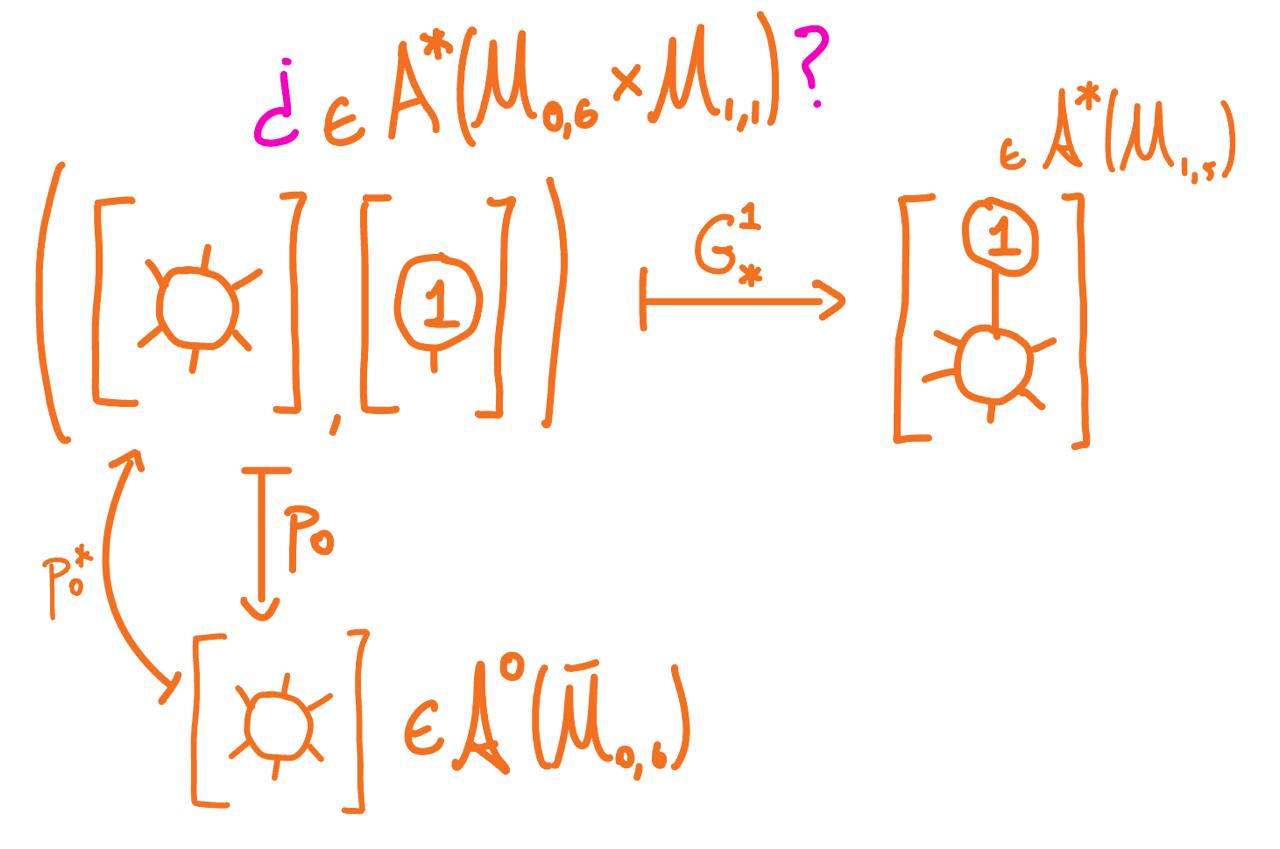
\includegraphics[width=0.5\textwidth, clip]{figs/GluingMapActionEx}
    \end{figure}
    This means that the pushforward of the fundamental class through $\cG^1$ is the class of curves described by the dual graph on the right of the diagram.\footnote{This sentence sounds a bit fishy. I just remember what you said about ``I can't pick a concrete representative''.}\par
    From this, we have 
    \begin{align*}
        (1+\la_1)\cG_\ast^1(\id)&=\cG_\ast^1(\id)+\la_1\cG_\ast^1(\id)\\
        &=\cG_\ast^1(\id)+\cG_\ast^1(p_1^\ast(\la_1))+\cG_\ast^1(p_0^\ast(\la_1))\\
        &=\cG_\ast^1(\id)+\cG_\ast^1(p_1^\ast(\la_1))+0.
    \end{align*}
    This quantity should be equal to $\cG^1_\ast(p_1^\ast(\La_1(1)))$, and expanding this we have
    \begin{align*}
        \cG^1_\ast(p_1^\ast(\La_1(1)))&=\cG^1_\ast(p_1^\ast(1+\la_1))\\
        &=\cG^1_\ast(p_1^\ast(1))+\cG^1_\ast(p_1^\ast(\la_1))\\
        &=\cG^1_\ast(1)+\cG^1_\ast(p_1^\ast(\la_1)),
    \end{align*}
    so both quantities are equal.\newpage
    Diagramatically we have 
    \begin{figure}[h]
        \centering
        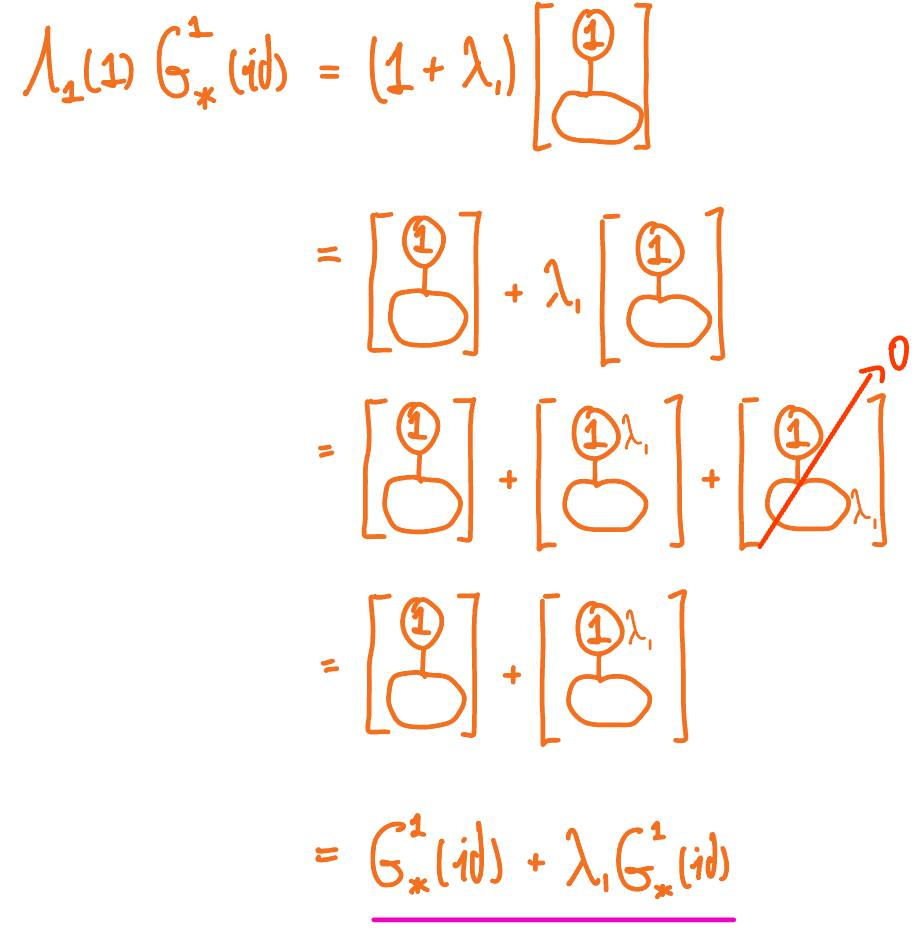
\includegraphics[width=0.5\textwidth, clip]{figs/DiagramGenus1TotChernG1PB}
    \end{figure}\\
    The calculation for $\cG^1_\ast(\id)\La_1(-1)$ is similar but different signs. Finally calculating $\cG_\ast^1(\id)^2$ amounts to finding a self intersection number.  
\end{Ex}

\begin{Qn}
    I remember how to find $E\cap E$ in $\Bl_{\text{pt}}\bP^2$ by deforming a cycle that goes through $E$. ¿Is the technique to find $\cG_\ast^1(\id)\cap \cG_\ast^1(\id)$ similar?
\end{Qn}

\section{A reconsideration on the Mumford formula}

\chapter{A bit of Algebra}

\section{Schemes}

I'm lacking a bit on the side of what schemes are. The definition we have is as follows:

\begin{Def}
    An affine scheme is a topological space $X$ which is isomorphic to an irreducible algebraic subset of $k^n$, together with a sheaf of $k$-valued functions $\cO_X$.
\end{Def}

All of the words here make sense, right? So let's do some examples:

\begin{Ex}
    Consider the space $\Spec\bZ$
\end{Ex}

\chapter{II2025 - The space of maps}

\section{The Faber-Pandharipande formula for multiple covers}

We are interested in calculating the Gromov-Witten invariant\footnote{Whatever a GW invariant is, one of its many manisfestations is as an integral.}
$$\int_{[\ov{\cM}_{g,0}(X,d\bt)]^\vir}1.$$
Here, $X$ is a Calabi-Yau threefold and $\bt$ represents the class of a line. The moduli space then parametrizes maps from $\ov{\cM}_g$ to a Calabi-Yau which land on a line and such map has degree $d$.\par
To this effect, we first deal with the examples in genus 0 known as the Aspinwall-Morrison formula. We illustrate this via examples.

\subsection{Degree 3}

 In degree 3 and genus 0 we have
$$\int_{[\ov{\cM}_{0,0}(X,3\bt)]^\vir}1=(\deg.\ 3\ \text{inmersions})+(\deg.\ 3\ \text{covers of }\bt).$$
The part that we may calculate consists of the triple covers of the line $\bt$. Such integral is actually
$$\int_{\ov{M}_{0,0}(\bP^1,3)}1$$
and the (virtual) fundamental class is $e(\Ob)$ as our moduli space is non-singular. This comes from section 26.1.2 of the Mirror Symmetry book \cite{BigMirrorSymmetryBook}. For a map $[(C,f)]\in\cM$ (we now abbreviate the moduli space into $\cM$), we have the following tangent-normal sequence
$$0\to TC\hookto f^\ast TX\onto N_{C\mid X}\to 0$$
which, after applying $H^\ast(C,-)$, becomes
$$
    \begin{tikzcd}
  H^0(C,TC) \rar & H^0(C,f^\ast TX) \rar
             \ar[draw=none]{d}[name=X, anchor=center]{}
    & H^0(C,N_{C\mid X}) \ar[rounded corners,
            to path={ -- ([xshift=2ex]\tikztostart.east)
                      |- (X.center) \tikztonodes
                      -| ([xshift=-2ex]\tikztotarget.west)
                      -- (\tikztotarget)}]{dll}[at end]{} \\   
 H^1(C,TC) \rar & H^1(C,f^\ast TX) \rar
             \ar[draw=none]{d}[name=Y, anchor=center]{}
    & H^1(C,N_{C\mid X}) \ar[rounded corners,
            to path={ -- ([xshift=2ex]\tikztostart.east)
                      |- (Y.center) \tikztonodes
                      -| ([xshift=-2ex]\tikztotarget.west)
                      -- (\tikztotarget)}]{dll}[at end]{} \\      
  H^2(C,TC) =0 &\phantom{cuminmyass}&
\end{tikzcd}
$$
Via deformation theory, this sequence is actually
  $$
    \begin{tikzcd}
  \Aut(C)\rar & \DefB(f) \rar
             \ar[draw=none]{d}[name=X, anchor=center]{}
    & \DefB(C,f)\ar[rounded corners,
            to path={ -- ([xshift=2ex]\tikztostart.east)
                      |- (X.center) \tikztonodes
                      -| ([xshift=-2ex]\tikztotarget.west)
                      -- (\tikztotarget)}]{dll}[at end]{} \\   
 \DefB(C)\rar & \Ob(f) \rar
    & \Ob(C,f) 
\end{tikzcd}
$$
And lemma 24.4.3 of \cite{BigMirrorSymmetryBook} guarantees that for our map $f\: C\to\bP^1$ we have $h^1(C,f^\ast T\bP^1)=0$ because $C$ is a genus 0 curve. In consequence
$$\Ob(f)\isom H^1(C,N_{C\mid X})$$
and in order for this to be a bundle over our source, we pull it back via $f$. 

\begin{Prop}
    Given our conditions, $X$ being Calabi-Yau, the bundle $N_{C\mid X}$ is a rank $2$ vector bundle of degree $-2$.
\end{Prop}

\begin{ptcbp}
    The rank can be seen inmediately to be two as the dimension of $C$ inside $X$ is $1$, so it has codimension $2$. For the degree, using the same tangent-normal sequence for $f\: C\to X$ we have 
    $$0\to TC\hookto f^\ast TX\onto N_{C\mid X}\to 0$$
    and $TC\isom\cO(2)$. Taking first Chern class we get
    $$c_1(f^\ast TX)=c_1(TC)+c_1(N_{C\mid X}).$$
    As $X$ is Calabi-Yau, $c_1(TX)=0$ and so 
    $$0=2+c_1(N_{C\mid X})$$
    so that the degree of $N_{C\mid X}$ is $-2$, the degree of its first Chern class.
\end{ptcbp}

Such a bundle splits into a direct sum 
$$N_{C\mid X}\isom L_1\oplus L_2=\cO(d_1)\oplus\cO(d_2)$$
and being of degree $-2$ means that $d_1+d_2=-2$. A theorem due to Grothendieck\footnote{God knows which} states that such distribution must be as balanced as possible so that $d_1=d_2=-1$. In conclusion
$$e(\Ob)=e(H^1(C,f^\ast N_{C\mid X}))=e(H^1(C,f^\ast\cO(-1)^2)).$$
Our target integral along with the expected result via Aspinwall-Morrison's result is
$$\int_{\ov{M}_{0,0}(\bP^1,3)}e(H^1(C,f^\ast\cO(-1)^2))=\frac{1}{3^3}.$$
Via localization, as the torus action $t\.x=tx$ extends naturally from $\bP^1$ to $\cM$, we have $7$ fixed loci:

%what is up my pex

\begin{figure}[h!]
        \centering
        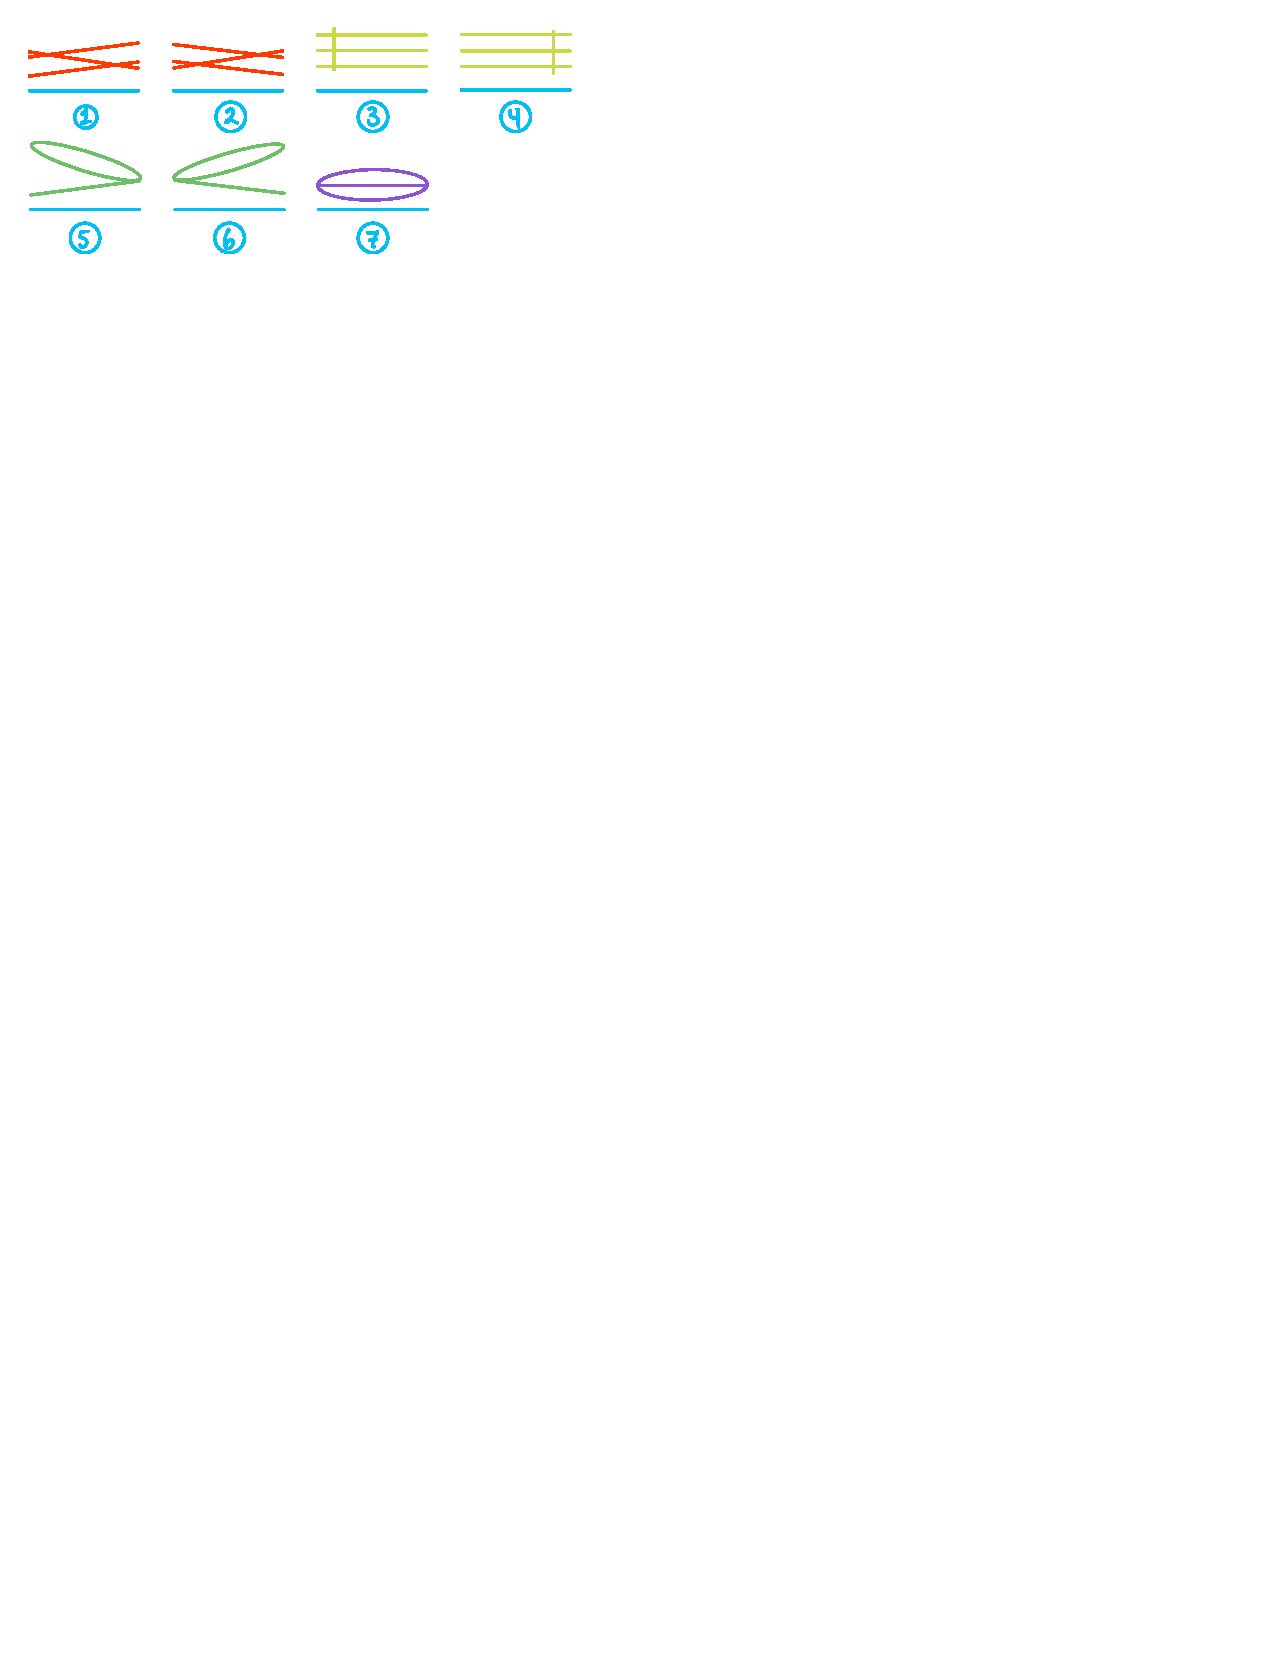
\includegraphics[width=0.8\textwidth, trim= 0.1cm 24cm 9cm 0.1cm,clip]{figs/FigsDNnotability5.pdf}
        \caption{Fixed loci of $\cM$ (uhhhh)}
        \label{fig:6.1-fixed-loci-maps-g0-d3}
    \end{figure} 

The calculation for odd numbered fixed loci is the same as even numbered so we only do the calculation for the odd ones.\par

\textbf{Fixed locus 1:} Consider the first fixed loci representing a rational curve with two nodes, each $\bP^1$ maps with degree 1 to the base. The normalizaiton sequence for this curve is 
$$0\to\cO_C\to\cO_{C_1}\oplus\cO_{C_2}\oplus\cO_{C_3}\to\bC_{n_1}\oplus\bC_{n_2}\to0$$
where $\cO_{C_i}$ is the trivial sheaf of the $i^{\text{th}}$ component of the curve $C$. The $\bC_{n_i}$ correspond to skyscraper sheaves over the nodes. The numbering of the normalization sequence goes from bottom to top.

\begin{Qn}
    What are the maps in this normalization sequence?
\end{Qn}

Tensoring the sequence via $-\ox f^\ast\cO(-H)$ we obtain 
$$0\to f^\ast\cO(-H)\to\cO(-H)^3\to \genr{(0)}\oplus\genr{(-t)}\to 0$$
and then taking the long exact sequence in cohomology $H^\ast(C,-)$ we get 
$$
\begin{tikzcd}[column sep=tiny, row sep=tiny]
0 \arrow[r] &
H^0(f^\ast \cO(-H)) \arrow[r] &
H^0(\cO(-H))^3 \arrow[r] &
H^0(\genr{(-t)}) \oplus H^0(\genr{(0)})
  \ar[rounded corners, to path={ -- ([xshift=2ex]\tikztostart.east) |- (X.center) \tikztonodes -| ([xshift=-2ex]\tikztotarget.west) -- (\tikztotarget)}]{dll}[at end]{}\\[1ex]
& H^1(f^\ast \cO(-H)) \arrow[r] &
H^1(\cO(-H))^3 \arrow[r] &
0
\end{tikzcd}
$$
Observe that the first two terms are zero because the bundle is negative. By Serre duality:
$$h^1(\cO(-1))=h^0(K_{\bP^1}\ox\cO(-1)^{\vee})=h^0(\cO(-2)\ox\cO(1))=h^0(\cO(-1))=0.$$
Finally the last term corresponding to the $H^1$ of the skyscrapers is zero because of dimension vanishing. The sequence becomes
$$0\to H^0(\genr{(-t)}) \oplus H^0(\genr{(0)}) \to H^1(f^\ast \cO(-H))\to0$$
and taking Euler classes returns
$$e( H^1(f^\ast \cO(-H)))=e(H^0(\genr{(-t)}))e(H^0(\genr{(0)}))=(-t)(0).$$
Immediately the integral is zero for this and the second fixed loci. It is possible to calculate its normal bundle's Euler class, but we reserve that for the next maps.\par
\textbf{Fixed locus 3:}\par
The normalization sequence is now 
$$0\to\cO_C\to\bigoplus_{i=1}^{4}\cO_{C_i}\to\bigoplus_{i=1}^{3}\bC_{n_i}\to0$$
Here $C_4$ is the curve connecting the other $3$ $\bP^1$'s. Tensoring $-\ox f^\ast\cO(-H)$ we obtain 

$$0\to f^\ast\cO(-H)\to\cO(-H)^3\oplus\cO(-t)\to \genr{(-t)}^3\to 0$$

where $\cO(-t)$ is the copy of the fiber above $0$ at every point of the collapsed $\bP^1$. The pullback takes a copy of the fiber over zero and puts it over every point of that $\bP^1$ giving us the trivial sheaf in question.\par
Taking now long exact sequence in cohomology $H^\ast(C,-)$ we obtain 
$$
\begin{tikzcd}[column sep=tiny, row sep=tiny]
0 \arrow[r] &
H^0(f^\ast \cO(-H)) \arrow[r] &
H^0(\cO(-H))^3\oplus H^0(\cO(-t)) \arrow[r] &
H^0(\genr{(-t)})^3
  \ar[rounded corners, to path={ -- ([xshift=2ex]\tikztostart.east) |- (X.center) \tikztonodes -| ([xshift=-2ex]\tikztotarget.west) -- (\tikztotarget)}]{dll}[at end]{}\\[1ex]
& H^1(f^\ast \cO(-H)) \arrow[r] &
H^1(\cO(-H))^3\oplus H^1(\cO(-t)) \arrow[r] &
0
\end{tikzcd}
$$
Cancelling some terms we are left with
$$0\to H^0(\cO(-t))\to H^0(\genr{(-t)})^3\to H^1(f^\ast \cO(-H))\to 0.$$
The first cohomology of the trivial bundle cancels because by Serre duality it has dimension $h^0(\cO(-2))=0$. The Euler class is thus 
$$H^1(f^\ast \cO(-H))=\frac{(-t)^3}{-t}=t^2$$
however when linearizing with $\cO(-H+t)$ all the weights in question become zero. So that the numerator ends up being zero altogether. Same reasoning applies to the fourth fixed loci.\par
\textbf{Fixed locus 5:}\par
The normalization sequence is 
$$0\to\cO_C\to\cO_{C_1}\oplus\cO_{C_2}\to\bC_{n}\to0$$
and observe that when pulling back $\cO(-H)$ to $C_2$ it pulls back with the same weights $-t$ and $0$. With respect to $C_2$'s hyperplane class, say $\widetilde{H}$ whose weights for $\cO(-\widetilde{H})$ are $\frac{-t}{2}$ and $0$, the pullback becomes $\cO(-2\widetilde{H})$. So the result of applying $-\ox f^\ast\cO(-H)$ is
$$0\to f^\ast\cO(-H)\to\cO(-H)\oplus\cO(-2\widetilde{H})\to \genr{(0)}\to 0.$$
We then take long exact sequence in cohomology $H^\ast(C,-)$:
$$
\begin{tikzcd}[column sep=tiny, row sep=tiny]
0 \arrow[r] &
H^0(f^\ast \cO(-H)) \arrow[r] &
H^0(\cO(-H))\oplus H^0(\cO(-2\widetilde{H})) \arrow[r] &
H^0(\genr{(0)})
  \ar[rounded corners, to path={ -- ([xshift=2ex]\tikztostart.east) |- (X.center) \tikztonodes -| ([xshift=-2ex]\tikztotarget.west) -- (\tikztotarget)}]{dll}[at end]{}\\[1ex]
& H^1(f^\ast \cO(-H)) \arrow[r] &
H^1(\cO(-H))\oplus H^1(\cO(-2\widetilde{H})) \arrow[r] &
0
\end{tikzcd}
$$
Immediately the first two terms cancel out because of negative degree and one $H^1$ cancels due to Serre duality. We are left with the sequence 
$$0\to H^0(\genr{(0)})\to H^1(f^\ast \cO(-H))\to H^1(\cO(-2\widetilde{H}))\to 0.$$
Observe that the middle section of $H^1(\cO(-2\widetilde{H}))$ has weight $\frac{-t}{2}$. This comes from the formula 
$$
\left\lbrace
\begin{aligned}
&w_0-w_\infty=(\deg.)w_{0,TX}\To w_0 - (\deg.)w_{0,TX}\\
&-t-0=(-2)\left(\frac{t}{2}\right)\To -t-(-2)\left(\frac{t}{2}\right)=0.
\end{aligned}
\right.
$$
The middle section then has weight 

$$-t-(-1)\left(\frac{t}{2}\right)=-t+\frac{t}{2}=\frac{-t}{2}$$

Thus the whole Euler class for our desired bundle is 
$$e(H^1(f^\ast \cO(-H)))=(0)\left(\frac{-t}{2}\right)=0.$$
\begin{Ej}
    The Euler class for the other linearization $\cO(-H+t)$ ends up being
$$e(H^1(f^\ast \cO(-H+t)))=(t)\left(\frac{t}{2}\right).$$
\end{Ej}

Multiplying both classes returns $0$ and thus the integral is zero. The remaining fixed locus is the only one with a non-zero contribution to the integral.\par
\textbf{Fixed locus 7:}\par 
There's no need to apply a normalization sequence argument as there's only one component. We directly ask for $H^1(f^\ast(\cO(-H)))$. In this case $\cO(-H)$ pulls back to a $\cO(-3\widetilde{H})$ where $\widetilde{H}$ is the hyperplane class of the curve $C_7$. $H^1(\cO(-3\widetilde{H}))$ has 2 middle sections with weights
$$w_0-w_{\tan},\word{and}w_0-2w_{\tan}.$$
These are 
$$-t-(-1)\left(\frac{t}{3}\right),\word{and}-t-(-2)\left(\frac{t}{3}\right)$$
so that the resulting Euler class is 
$$e(H^1(f^\ast(\cO(-H))))=\left(\frac{-2t}{3}\right)\left(\frac{-t}{3}\right)=\frac{2t^2}{9}.$$
In an analogous fashion, $f^\ast\cO(-H+t)$ coincides with $C_7$'s $\cO(-3\widetilde{H}+t)$. It's two middle sections have weights
$$w_\infty+w_{\tan},\quad w_\infty+2w_{\tan}\word{which are}t+(-1)\frac{t}{3},\quad t+(-2)\frac{t}{3}$$
so that 
$$i^\ast_7\left(e(H^1(f^\ast(\cO(-H))))e(H^1(f^\ast(\cO(-H+t))))\right)=\frac{2t^2}{9}\.\frac{2t^2}{9}=\frac{4t^4}{81}.$$
\begin{Rmk}
    The key difference between this locus and the others is that the $H^1$ contribution only considers the \emph{middle} sections which have non-zero weights. In the other cases, the extremes are taken, and one of those weights is zero. 
\end{Rmk}
We now proceed by considering the normal bundle of $F_7$ inside $\cM$. The dual graph of $C_7$ consists of an edge with label $3$ connecting two vertices. Such valence 1 vertices contribute each their corresponding tangent weight to automorphism bundle's Euler class:
$$e(\Aut(C_7))=\left(\frac{t}{3}\right)\left(\frac{-t}{3}\right)=\frac{-t^2}{9}.$$
The curve $C_7$ has no deformations as it is smooth. And finally looking at the deformations of the map
$$\DefB(f)=H^0(C_7,f^\ast T\bP^1)$$
which we identify to $\cO(2\.3\widetilde{H}-t)$ with respect to $\widetilde{H}$. This $\cO(6)$ has $7$ global sections with weights $w_0-kw_{\tan}$ with $0\leq k\leq \deg\cO(6)$, these are
$$t,\frac{2t}{3},\frac t3,0,-\frac t3,-\frac{2t}{3},-t.$$
The one with zero weight corresponds to a fixed section so we don't take that into account of the \emph{moving part} of the Euler class. We get
$$e(\DefB(f_7))=\frac{-4t^6}{81}\To e(N)=\frac{4t^6}{81}\left(\frac{-t^2}{9}\right)^{-1}=\frac{4t^4}{27}.$$
\begin{Rmk}
    We have that $e(N)$'s degree coincides with the codimension of $F_7$ inside of $\cM$. The dimension of $\ov{M}_{0,0}\left(\bP^1,3\right)$ is 
    $$(1+1)(3+1)+(0-3)-1=8-3-1=4$$
    which coincides with our observation that $F_7$ is a point (or a zero-dimensional scheme) inside $\cM$.
\end{Rmk}

Finally putting this together we have that 

$$\int_{\ov{M}_{0,0}(\bP^1,3)}e(\Ob)=0+\dots+0+\frac13\int_{F_7}\frac{i_7^\ast(e\.e)}{e(N_{F_7\mid\cM})}=\frac{{4t^4}/{81}}{{4t^4}/{27}}=\frac13\.\frac19=\frac{1}{27}$$

as expected.
%%%%%%%%%%%% Contents end %%%%%%%%%%%%%%%%
\ifx\nextra\undefined
\printindex
\else\fi
\nocite{*}
\bibliographystyle{plain}
\bibliography{bibiDoctoralNotebook.bib}
%https://anddil.github.io/teaching/ %moduli of curves and maps
%https://www.math.colostate.edu/~renzo/teaching/Toric18/Linebundles.pdf %Renzo LBS
\end{document} 

